\documentclass[12pt]{article}
\usepackage{amsmath,amssymb,latexsym}
\usepackage{graphicx,psfrag,epsf}
\usepackage{enumerate}
\usepackage{natbib}
\usepackage{wrapfig}
\usepackage{subcaption}
\usepackage{listings}
\usepackage{xcolor}
\usepackage{booktabs} 
\usepackage{array}

\definecolor{codegreen}{rgb}{0,0.6,0}
\definecolor{codegray}{rgb}{0.5,0.5,0.5}
\definecolor{codepurple}{rgb}{0.58,0,0.82}
\definecolor{codeyellow}{rgb}{0.51, 0.37, 0.012}

\lstset{
    aboveskip=\baselineskip,
  commentstyle=\color{codegreen},
  keywordstyle=\bfseries\color{codeyellow},
  numberstyle=\ttfamily\tiny\color{codegray},
  stringstyle=\color{codepurple},
  basicstyle=\ttfamily\footnotesize,
  breakatwhitespace=false,
  breaklines=true,
  captionpos=b,
  keepspaces=true,
  numbers=left,
  xleftmargin=2em,
  numbersep=5pt,
  showspaces=false,
  showstringspaces=false,
  showtabs=false,
  tabsize=2,
  frame=tb
    }

\newcommand{\blind}{0}

\addtolength{\oddsidemargin}{-.75in}%
\addtolength{\evensidemargin}{-.75in}%
\addtolength{\textwidth}{1.5in}%
\addtolength{\textheight}{1.3in}%
\addtolength{\topmargin}{-.8in}%
\pagenumbering{gobble}

\begin{document}
\pagenumbering{arabic}

%\bibliographystyle{natbib}

\def\spacingset#1{\renewcommand{\baselinestretch}%
{#1}\small\normalsize} \spacingset{1}



%%%%%%%%%%%%%%%%%%%%%%%%%%%%%%%%%%%%%%%%%%%%%%%%%%%%%%%%%%%%%%%%%%%%%%%%%%%%%%

\if0\blind
{
  \title{\bf{Sport Analysis} \\ \small{The prediction of the final credits and each game scores of the Premier League} }
  \author{Stanley Zheng \quad Gefei Wu \quad Zhengtao Zhang \quad Yufanxing Liu \quad Zihao Zhang\footnote{\textbf{Stanley Zheng}: Conceptualization, Methodology, Software, Data Curation, Investigation, Formal analysis, Writing, Supervision, Project administration. \textbf{Gefei Wu}: Methodology, Software, Investigation, Formal analysis. \textbf{Zhengtao Zhang}: Data Curation. \textbf{Yufanxing Liu}: Methodology, Software. \textbf{Zihao Zhang}: Methodology.}}
  \maketitle
} \fi

\if1\blind
{
  \bigskip
  \bigskip
  \bigskip
  \begin{center}
    {\LARGE\bf Title}
\end{center}
  \medskip
} \fi

\bigskip
\begin{abstract}
This research utilizes sophisticated analytical tools, including Multiple Linear Regression (MLR) models and simulations, applied to an extensive ten-year dataset of English Premier League (EPL) seasons. Across five MLR models, Liverpool consistently emerges as the frontrunner for the current season's championship. The incorporation of Monte Carlo simulation and Poisson distribution enhances the analysis by providing nuanced insights into likely score differentials for individual matches, contributing to a comprehensive understanding of match dynamics. This study not only reaffirms Liverpool's favoritism for the EPL title but also significantly advances the field of football analytics, offering a detailed perspective on team performance and match-specific nuances. In essence, the research positions Liverpool as the prime candidate for EPL glory in the 23-24 season.
\end{abstract}


\spacingset{1.45}
\section{Introduction}
\label{sec:intro}
In the vast tapestry of global sports, football stands tall as a unifying force, drawing in an immense and diverse fan base. Our team takes pride in being an integral part of this dynamic community that shares an unwavering passion for the beautiful game. Amidst the multitude of football leagues, the English Premier League (EPL) emerges as a beacon of influence, where each match becomes a spectacle, captivating the hearts and minds of millions of fans worldwide. The burning anticipation of which club will emerge triumphant as the EPL champion becomes a narrative that unfolds with each thrilling match, igniting fervor and enthusiasm among spectators.

The analytical lens through which we examine the EPL season involves the sophisticated use of multivariable linear regressions (MLRs). This statistical approach allows us to meticulously scrutinize data spanning the last decade, enabling us to make informed predictions about the final point standings of each team at the conclusion of the ongoing season. The interconnectedness of these predictions with the overarching question of championship conquest adds a layer of intrigue to our analysis. Concurrently, alternative methodologies are employed to forecast goal tallies for both home and away teams in each match, further enriching our understanding of the potential outcomes.

This research embarks on a journey to unravel the complexities of the English Premier League's competitive landscape. Drawing on a thorough examination of historical data, our aim is to provide reasoned and insightful predictions for the current season, offering fans a nuanced perspective on each team's performance. Beyond the realm of passionate supporters, the practical implications of our findings extend to club managers, dedicated fans, and professionals in the burgeoning field of sports analytics. By shedding light on the potential trajectories and competitive dynamics within the English Premier League, our research strives to contribute valuable insights to the broader discourse surrounding the sport.


\section{Dataset}
The dataset comprehensively covers match statistics spanning the English Premier League (EPL) football matches. Each entry meticulously details specific match facets, encompassing vital information such as the match date, participating home and away teams, full-time goal counts (FTHG and FTAG for the home and away teams respectively), denoting the match outcome (FTR indicating H for home team win, A for away team win, and D for draw), as well as halftime goal tallies (HTHG and HTAG).

Moreover, the dataset encapsulates intricate betting odds provided by bookmakers, presenting probabilities for diverse outcomes including the likelihood of a home win (B365H), a draw (B365D), and an away win (B365A). This extensive repository doesn't limit itself to match results but also incorporates additional statistical insights such as shots on target (HST and AST for home and away teams respectively), contributing to a multifaceted understanding of match dynamics. Notably, the dataset spans an extensive timeline, encompassing data from the 2012-2013 season to the 2023-2024 season, offering a rich and comprehensive historical perspective on EPL match performances and betting trends.

You can see part of our raw data in Appendix.A.
\section{Implementation of MLR for Prediction of seasonal credits}

\subsection{Data Preprocessing}

Within the code(the first code block), a primary focus is dedicated to the initialization of a meticulously structured dataframe, named "total\_data\_12\_13," serving as the repository for comprehensive statistics pertaining to the English Premier League (EPL) season of 2012-2013. This foundational step involves the extraction and incorporation of unique team names, strategically placed as the initial column of the dataframe. To ensure an all-encompassing representation of team performance, an array of columns is meticulously crafted to encompass various statistical dimensions. These include essential metrics like wins (W), draws (D), losses (L), total goals scored (Agoal), total goals conceded (Lgoal), as well as performance indicators such as shots (S), shots on target (ST), fouls (F), corners (C), yellow cards (Y), and red cards (R). This comprehensive structure not only sets the stage for in-depth analysis but also lays the groundwork for a holistic understanding of team dynamics throughout the specified EPL season.

\begin{lstlisting}
# to-do
unique(data_12_13["HomeTeam"])
total_data_12_13 = as.data.frame(unique(data_12_13["HomeTeam"]))
names(total_data_12_13)[1] <- "Team"
column_names <- c("W","D", "L", "Agoal", "Lgoal", "S", 
                  "ST", "F", "C", "Y", "R")
new_columns <- data.frame(matrix(ncol = length(column_names), 
                          nrow = nrow(total_data_12_13)))
colnames(new_columns) <- column_names
total_data_12_13 <- cbind(total_data_12_13, new_columns)
total_data_12_13
\end{lstlisting}

Moving forward, the code(the second code block) is intricately designed to dissect the initial 16 matches of the season, placing a specific emphasis on calculating the number of wins for each participating team. This task is streamlined through the definition of a specialized function named "count\_win," strategically crafted to extract pertinent data pertaining to a specific team and subsequently tally the number of victories. The orchestration of this function is then executed through an iteration process, where the unique team names are systematically traversed. The culmination of this iterative journey results in the meticulous calculation and incorporation of the count of wins for each team, seamlessly populating the dedicated "W" column within the "total\_data\_12\_13" dataframe. This code segment not only lays the groundwork for subsequent analytical endeavors but also exemplifies a structured and purposeful approach towards extracting and utilizing critical match data for insightful outcomes.
\begin{lstlisting}
# win
count_win<-function(x){
    t = data_12_13[data_12_13$HomeTeam==x|
                 data_12_13$AwayTeam==x, ][1:16,]
    t1 = table(t[t$HomeTeam==x, ]$FTR)["H"]
    if (is.na(t1)) {
    t1 = 0
    }
    t2 = table(t[t$AwayTeam==x, ]$FTR)["A"]
    if (is.na(t2)) {
    t2 = 0
    }
    win = as.integer(t1 + t2)
    return(win)
}
team = unique(data_12_13["HomeTeam"])
team = team[,1]
W = c()
for (i in seq_along(team)) {
    res = count_win(team[i])
    W = c(W, res)
}
total_data_12_13$W = W
\end{lstlisting}
\subsection{Models}
As the Figure 1 showns, we use the history data to train our model, then we put the nowadays’ data into this model we trained, and then we get the prediction. This is how the data-driven model works.

\begin{figure}[h]
    \centering
    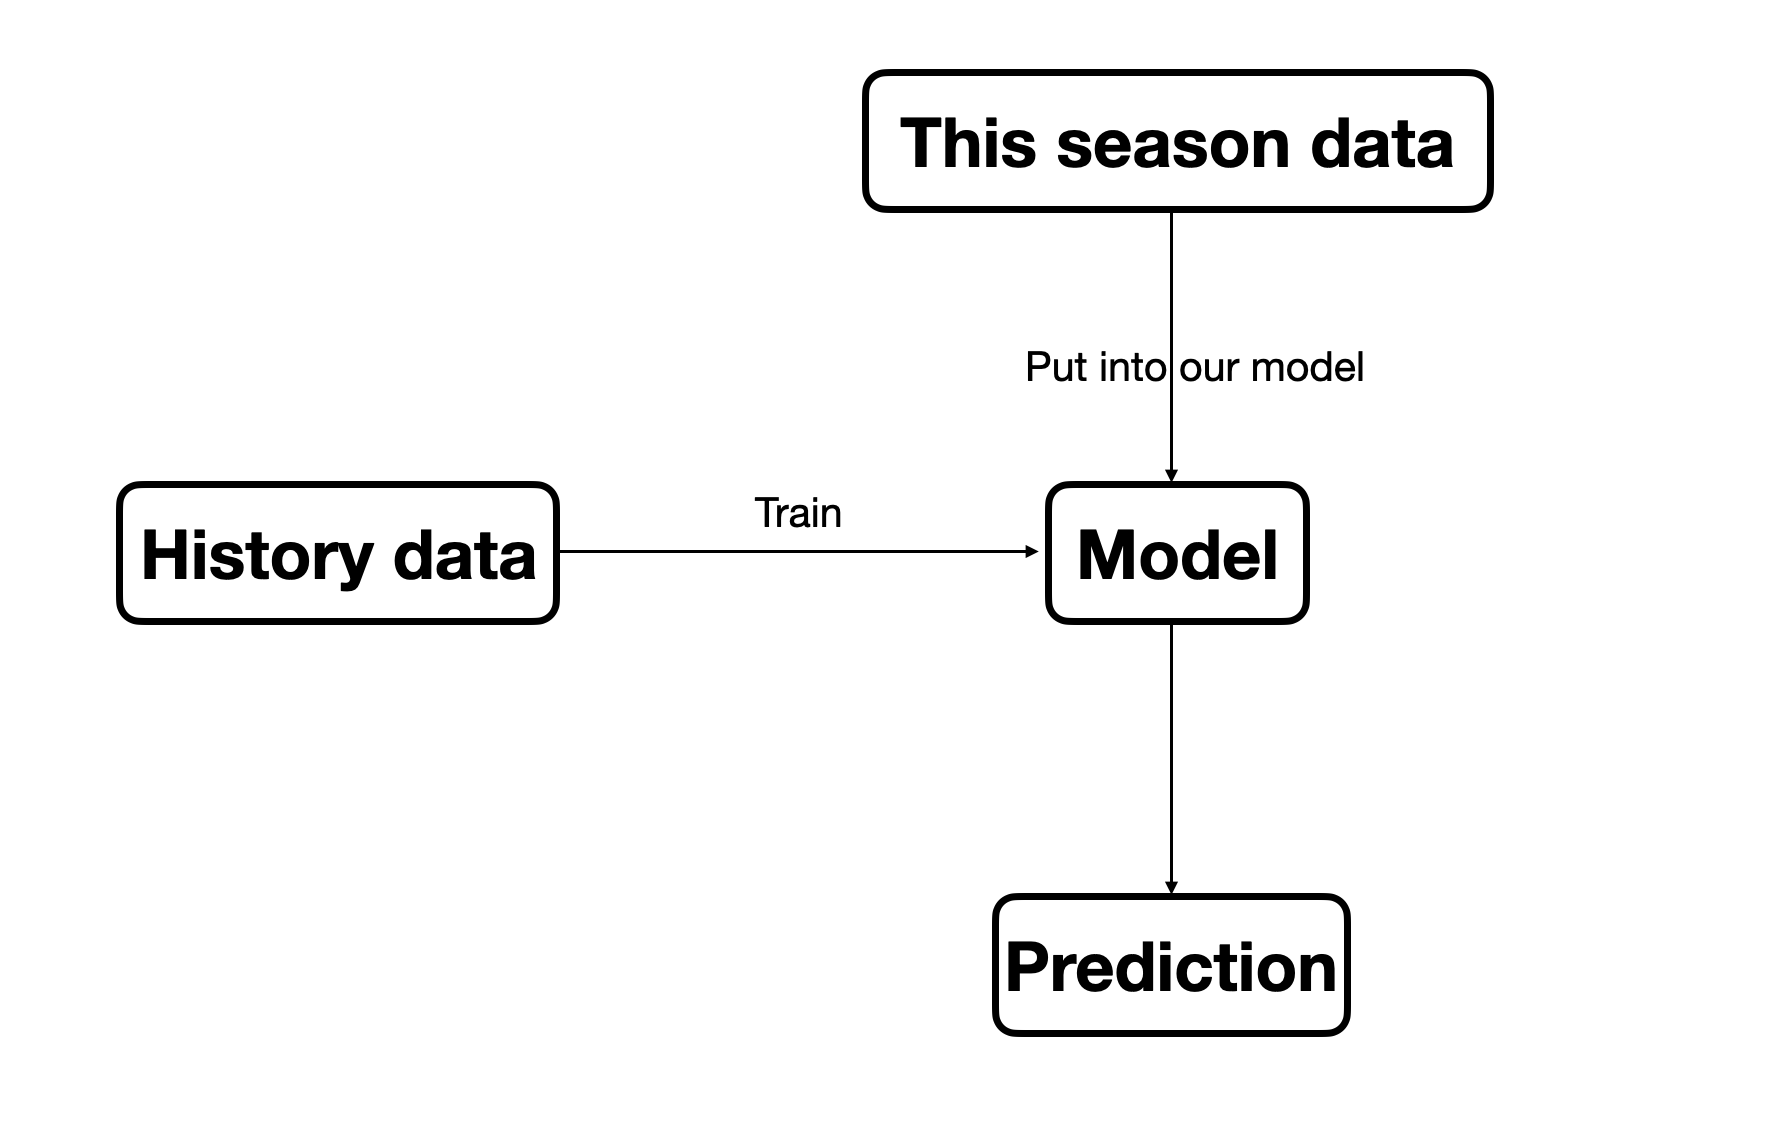
\includegraphics[width=0.6\linewidth]{1.png}
    \caption{Data-Driven Model.}
\end{figure}
The esstial point of our MLR models is that we only use the first 16th rounds to predict the final credits. We also only use the first 16th rounds data of the current season to predict final credits of the current season. This is like a mask, because in the end, when we use the data to predict, we only use the first 16th data, so to keep the consistency, when we train our data, even though we have the full data, we only use the first 16th round. This idea is as same as the idea of GPT in NLP area.

Now, we have the data we need, we can do the analysis. 

First, we just assumed that every explanatory variable could affect the final credits. And we apply end-to-end structure, which means we do no transformation to the explanatory variables or response variable. Then we just use the lm() function in R to get our multivariable linear regression models. The results you can see in Appendix.B. 

As we all know, we you use multivariable linear regression, it's actually build a high dimensional space, and try to find a hyperplane to fit our data point in this space. However, we know when the dimension increases, the data points we need increases exponentially. So, it's obvious that our data from last 10 seasons are not enough to support a 12 dimensional space. Intuitionally, this will lead to the "Curse of Dimensionality", Thus this, we need to reduce the dimension of our data. 

From the results of model1 we know W, D and S are the most related variables. We just keep these variable in our Model2.

Besides using the statistic way to decide which variable we should keep, we can apply some other methods. Like we can combine two variables into one index, and use this index to represent the original variable. Here, we combine the S and ST to get STR(Shoot-on-Target Rate), and we combine the Agoal and S to get GTR(Goal-on-Transfer Rate). The convert formula is 
$$
STR = \frac{ST}{S} \quad \quad GTR = \frac{Agoal}{S}.
$$
We also find that the value of R is very low, and only have very small amount of number. So, we just treat it as dummy variable. 

Nevertheless, we can see that the data we use are not on the same scale, so sometimes we think that the scale will also affect the results. Thus, we will do some normalization to the data.

In the Model3, I apply the Z-score normalization to our explanatory variables. The convert formula of Z-score normalization is 
$$
z_i = \frac{x_i - \Bar{x}}{\sigma_x}
$$

In the Model4, I apply the Min-Max normalization to our explanatory variables. The convert formula of Min-Max normalization is 
$$
x'_i = \frac{x_i - \text{Min}(x)}{\text{Max}(x)-\text{Min}(x)}
$$

In the Model5, I only make one change to Model4, which is I also apply the Min-Max normalization to the response variable.  

You can see the summaries of these give models in Appendix.B.
\subsection{Results}
From the summary of these models, we can compare the statistic indices between these models.

\begin{table}[h]
    \scriptsize 
    \centering
    \begin{tabular}{c m{8em}<{\centering} m{8em}<{\centering} m{8em}<{\centering} m{8em}<{\centering} m{9em}<{\centering}}
    \toprule
     & Model1 & Model2 & Model3 & Model4 & Model5\\
    \midrule
    Residual Standard Error & 7.081 on 208 DF & 7.092 on 216 DF& \multicolumn{2}{c}{7.285 on 206 DF} & 0.08673 on 206 DF  \\
    Multiple R-squared & 0.8519 & 0.8457& \multicolumn{3}{c}{0.8448}\\
    Adjusted R-squared & 0.8441 & 0.8436& \multicolumn{3}{c}{0.835}\\
    F-statistic & 108.8 on 11 &394.8 on 3 & \multicolumn{3}{c}{86.23 on 13}\\
    P-value & \multicolumn{5}{c}{$<2.2\times 10^{-16}$}\\
    \bottomrule
    \end{tabular}
    \caption{Statistic Indices}
\end{table}

The statistic indices in the Table 1 shows that, all these models have a very high R-squared and the P-values of theses models are very low. This means the model fit the sample points well, and these models all are reliable statistically. The residual standard error shows the bias between the real value and the prediction. You can see it's kind of high, since at the end of the season, even 1 credit can change the ownership of the champion. But in all model the residual standard error is already over 7 credits. In model 5, since we do some normalization to the credit, the range of the the converted credits is [0, 1], so in Model5 the residual standard error also relatively high. 

After we get these model, we can use these model to predict the final credits of each team at the end of this season. You can the prediction in Appendix.C. We can see the all five model predict that Liverpool. We only use first 16th round data, and now is the 20th round, Liverpool is actually on the top of the standings. Maybe it is the coincides, we will see the final results when the season over.


\section{Implementation of other models for the Prediction of scores}

\subsection{Data Preprocessing}
The code of data preprocessing snippet performs data preprocessing for football match data. It iterates through a list of file paths representing different seasons, reads CSV files, extracts relevant information, and calculates average goals for both home and away teams. The processed data is then stored, and all resulting data frames are combined into a single data frame. The final dataset is written to a CSV file named ``combined\_data.csv". The preprocessing includes handling column names, addressing team name variations, and aggregating match statistics.

The fully application you can find in the folder called ``Implementation of Monte Carlo simulation and Poisson distribution for the Prediction of scores".

\subsection{Model}
This model combines Monte Carlo simulation and Poisson distribution to predict football match outcomes. The function takes as input the home team, away team, the number of simulations, and historical match data. It selects the first 100 matches from the dataset for simulation, conducting 10,000 simulations for each match. 

In the simulation of each match, historical scoring averages drawn from the dataset are utilized to compute the average goals scored and conceded by both the home and away teams. This computation takes into consideration the amalgamation of historical data and overall team averages. Following this, through the application of the Poisson distribution, we generate random scores for the simulation. The resulting outcomes capture the most frequently occurring score and its corresponding probability.

The justification for employing Poisson distributions in modeling football scores stems from its aptitude in emulating the unpredictability of goal occurrences. The Poisson process, marked by its stationary, independent, and infrequent incremental nature, serves as an effective framework for mirroring the randomness inherent in goal events during football matches. By assuming that goals within short time intervals adhere to a Poisson distribution characterized by a rate parameter $\lambda$, this modeling approach adeptly encapsulates the essential aspects of sporadic and independent goal-scoring instances. As a result, it furnishes a practical approximation for the erratic nature of goal-scoring trends observed in football matches.

\subsection{Results}
In the specific code provided, the first 100 matches from the final\_data dataset are simulated, and the results are written to a CSV file named ``simulate\_outcome.csv." The probabilities in the prob column are divided by 100 to correct the scaling. Part of the results you can see in the Appendix.D.
\section{Discussion}
\label{sec:con}
In this comprehensive analysis of football match prediction models, our primary focus was on forecasting the English Premier League (EPL) champion for the current season. The foundational model, Multiple Linear Regression (MLR), demonstrated interpretability and ease of implementation. However, its reliance on a linear relationship between predictor variables and outcomes may oversimplify the intricate dynamics of football matches. To address this limitation, future iterations could explore the integration of non-linear models, such as polynomial regression or advanced machine learning algorithms like neural networks, to capture more nuanced patterns in the data.

Additionally, we employed Monte Carlo simulation and the Poisson distribution to predict match scores, providing a probabilistic outlook. While effective in offering a range of possible outcomes, this approach simplifies the complex interplay of factors influencing match results. Recommendations include exploring alternative probability distributions, such as the negative binomial distribution, to better account for overdispersion in the data. Moreover, expanding the scope beyond goal counts to incorporate additional features, like possession percentages or team strategies, could enhance the overall predictive accuracy.

Looking forward, our study suggests several avenues for model refinement. Experimentation with non-linear models and exploration of alternative probability distributions beyond Poisson can contribute to more accurate predictions. The incorporation of time-dependent variables and dynamic factors, such as player form and injuries, will likely improve model performance. Ensuring robustness through validation with out-of-sample data and addressing ethical considerations, such as potential biases in referee decisions, are crucial steps in advancing the reliability and fairness of football match prediction models. In conclusion, continuous refinement and the integration of advanced statistical techniques will be pivotal in developing models that provide nuanced and reliable insights into the unpredictable world of football.

\newpage

\section*{Appendix}

\section*{A. Dataset}
\label{Dataset}
\begin{figure}[h]
    \centering
    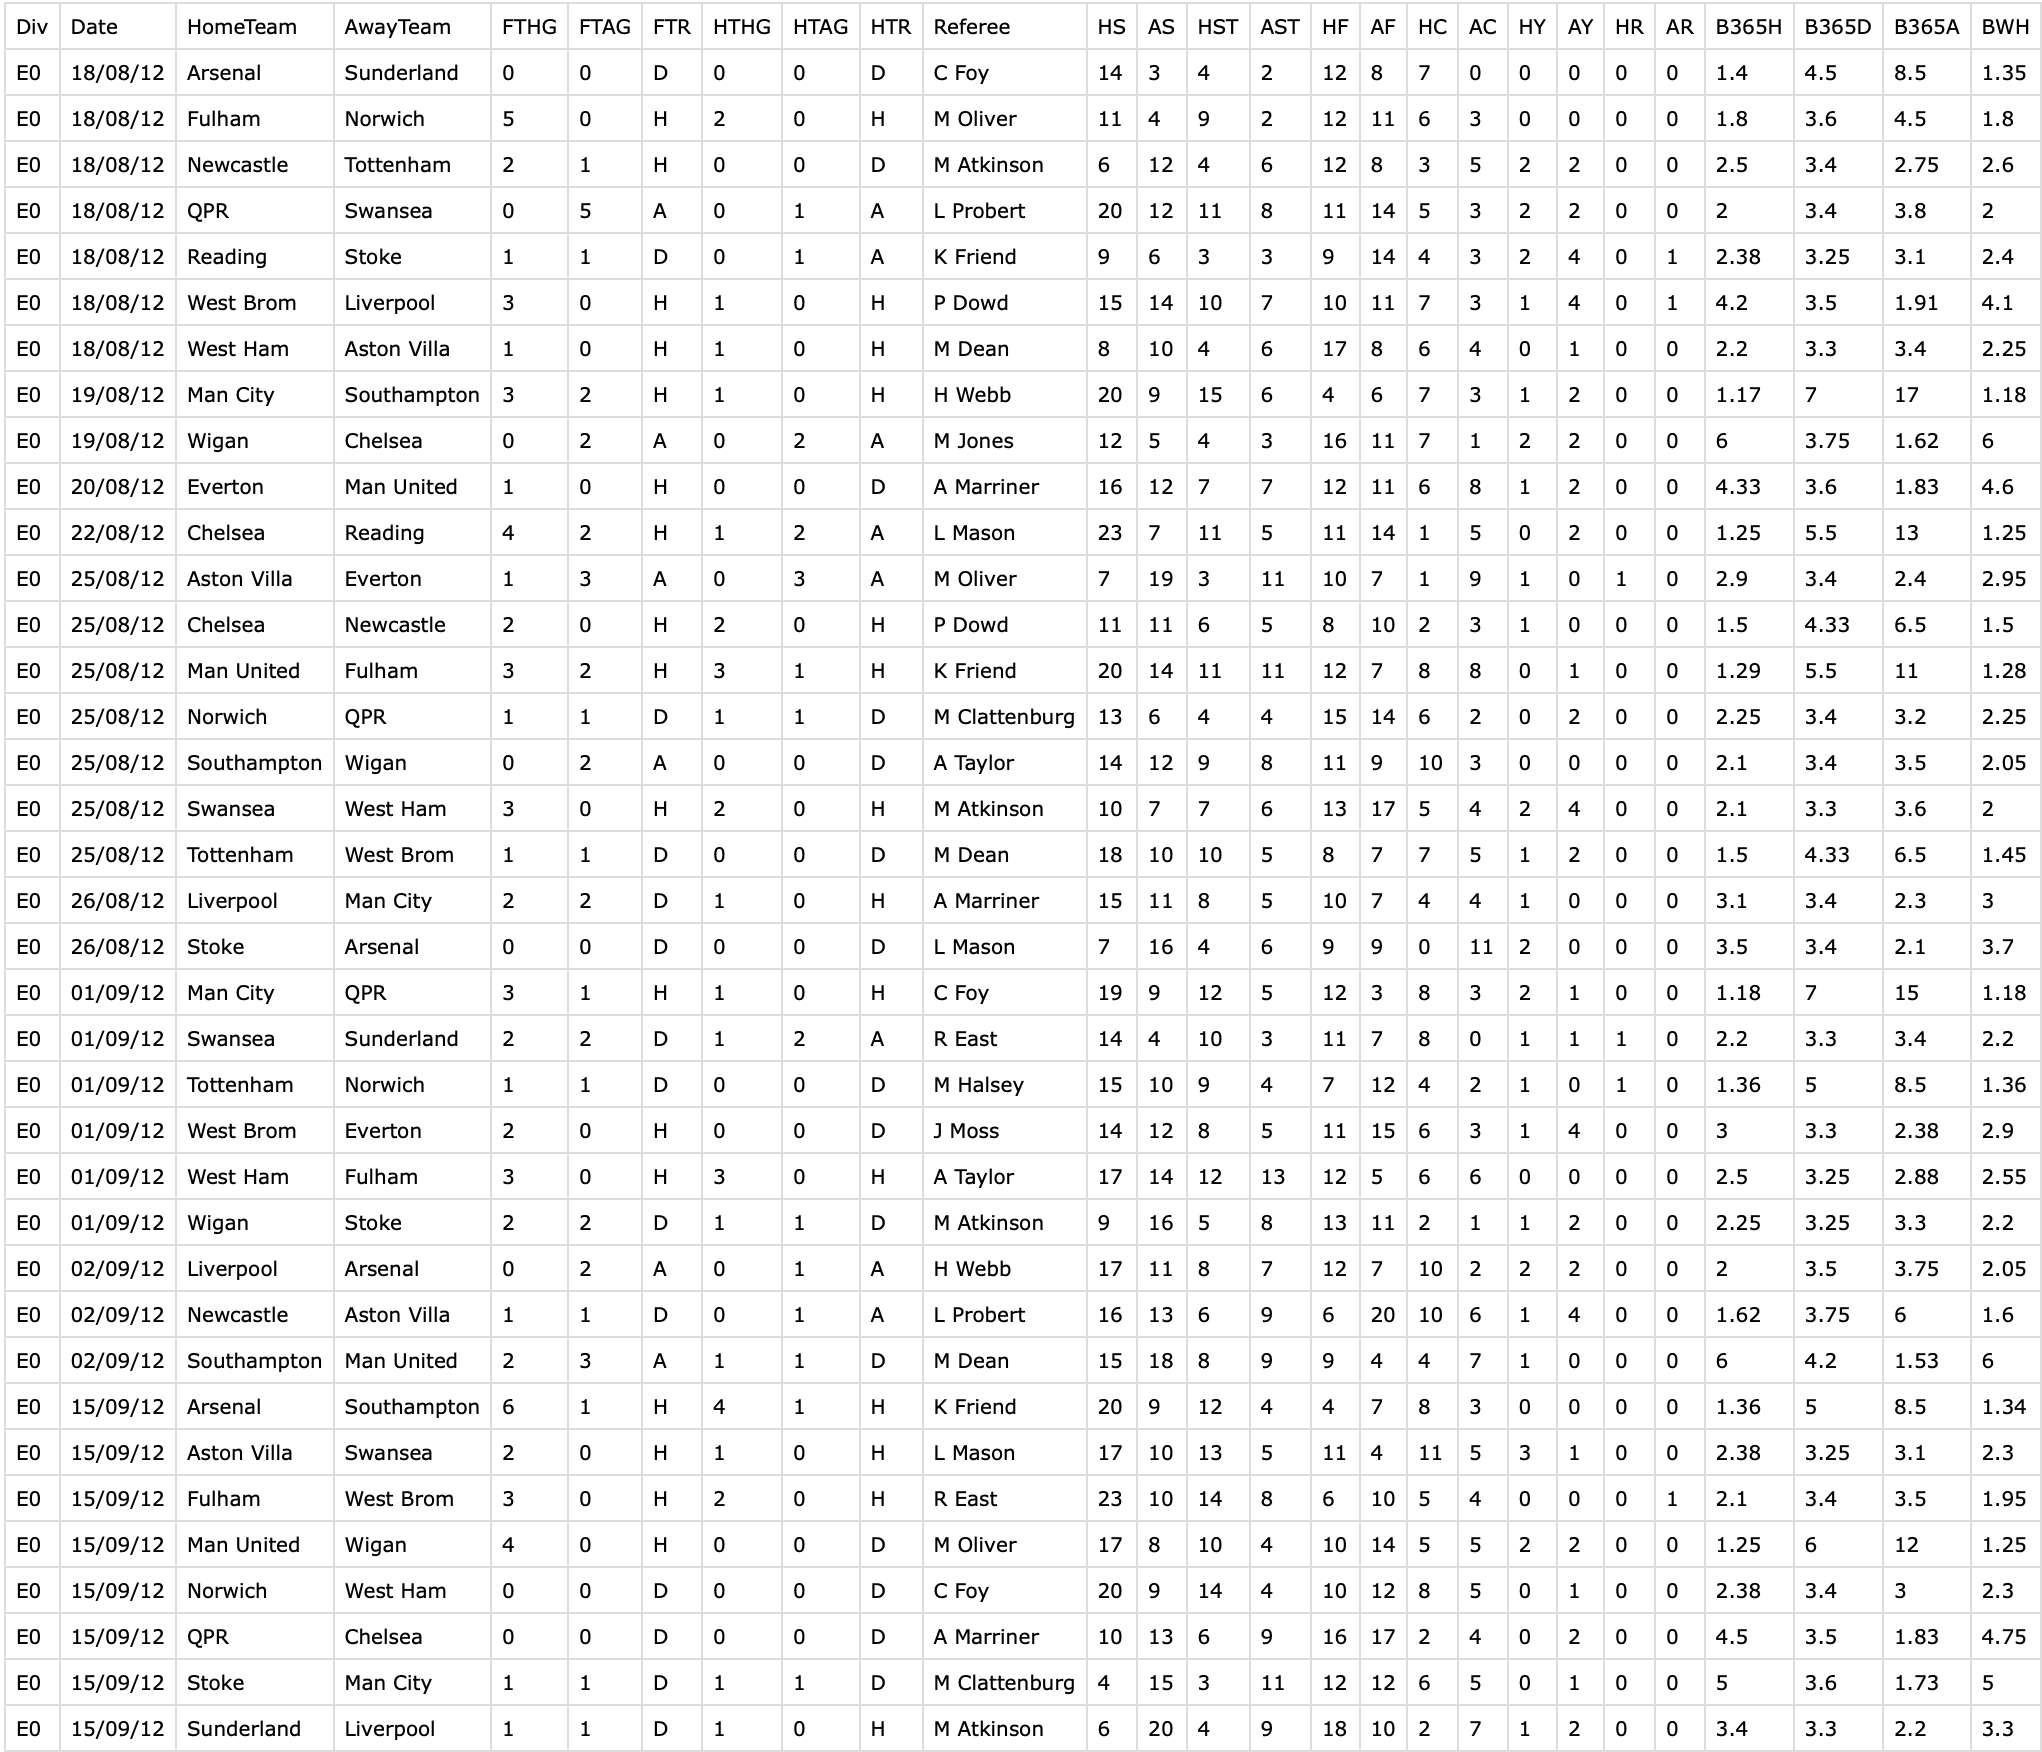
\includegraphics[scale=0.5]{Dataset.png}
    \caption{Dataset.}
\end{figure}

\newpage
\subsection*{B. MLR Model Results}
\label{Models}
\begin{figure}[h]
    \centering
    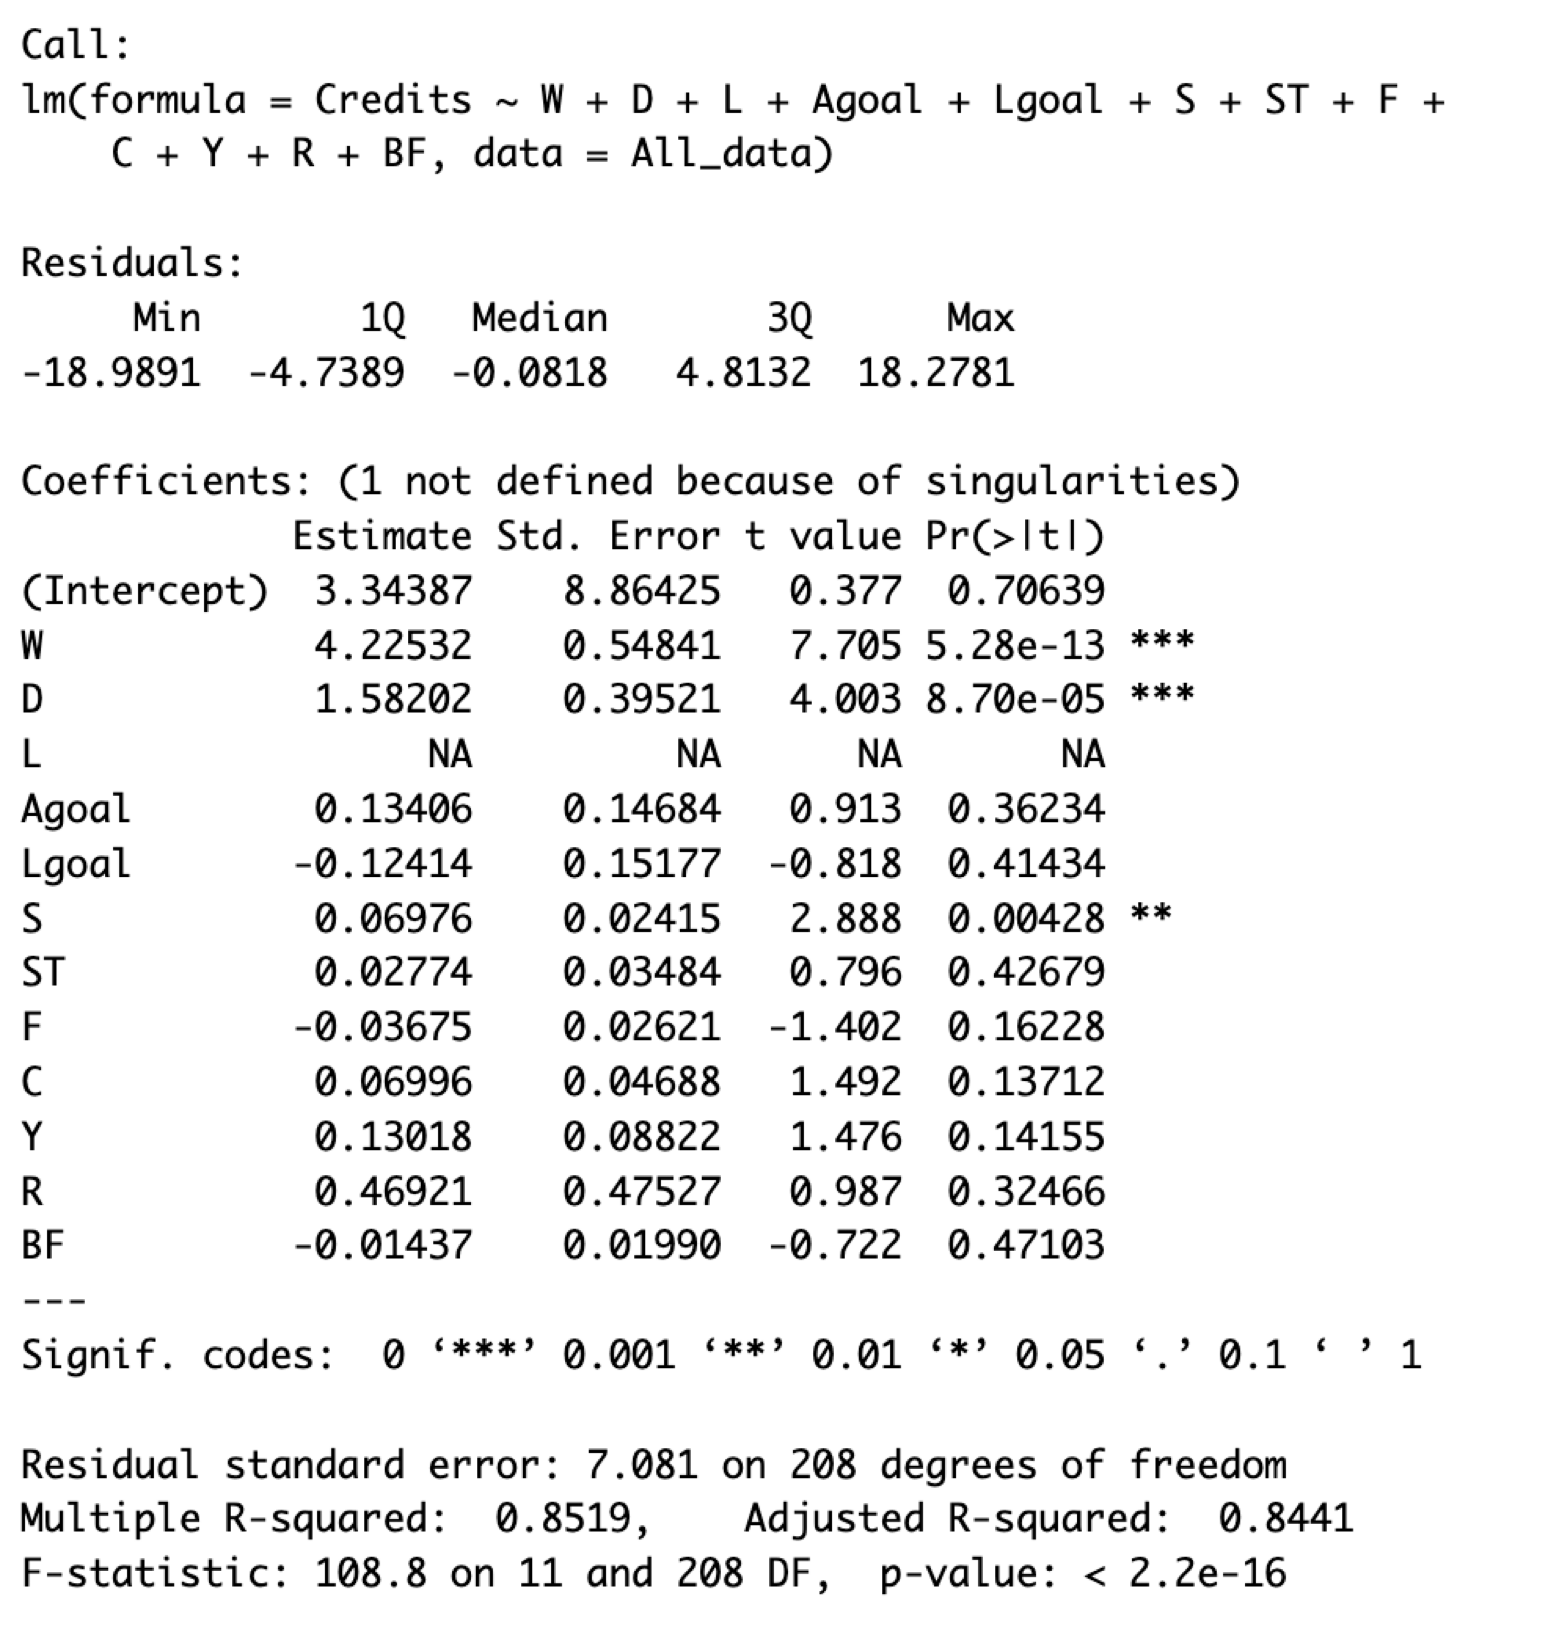
\includegraphics[width=0.32\linewidth]{m1.png}
    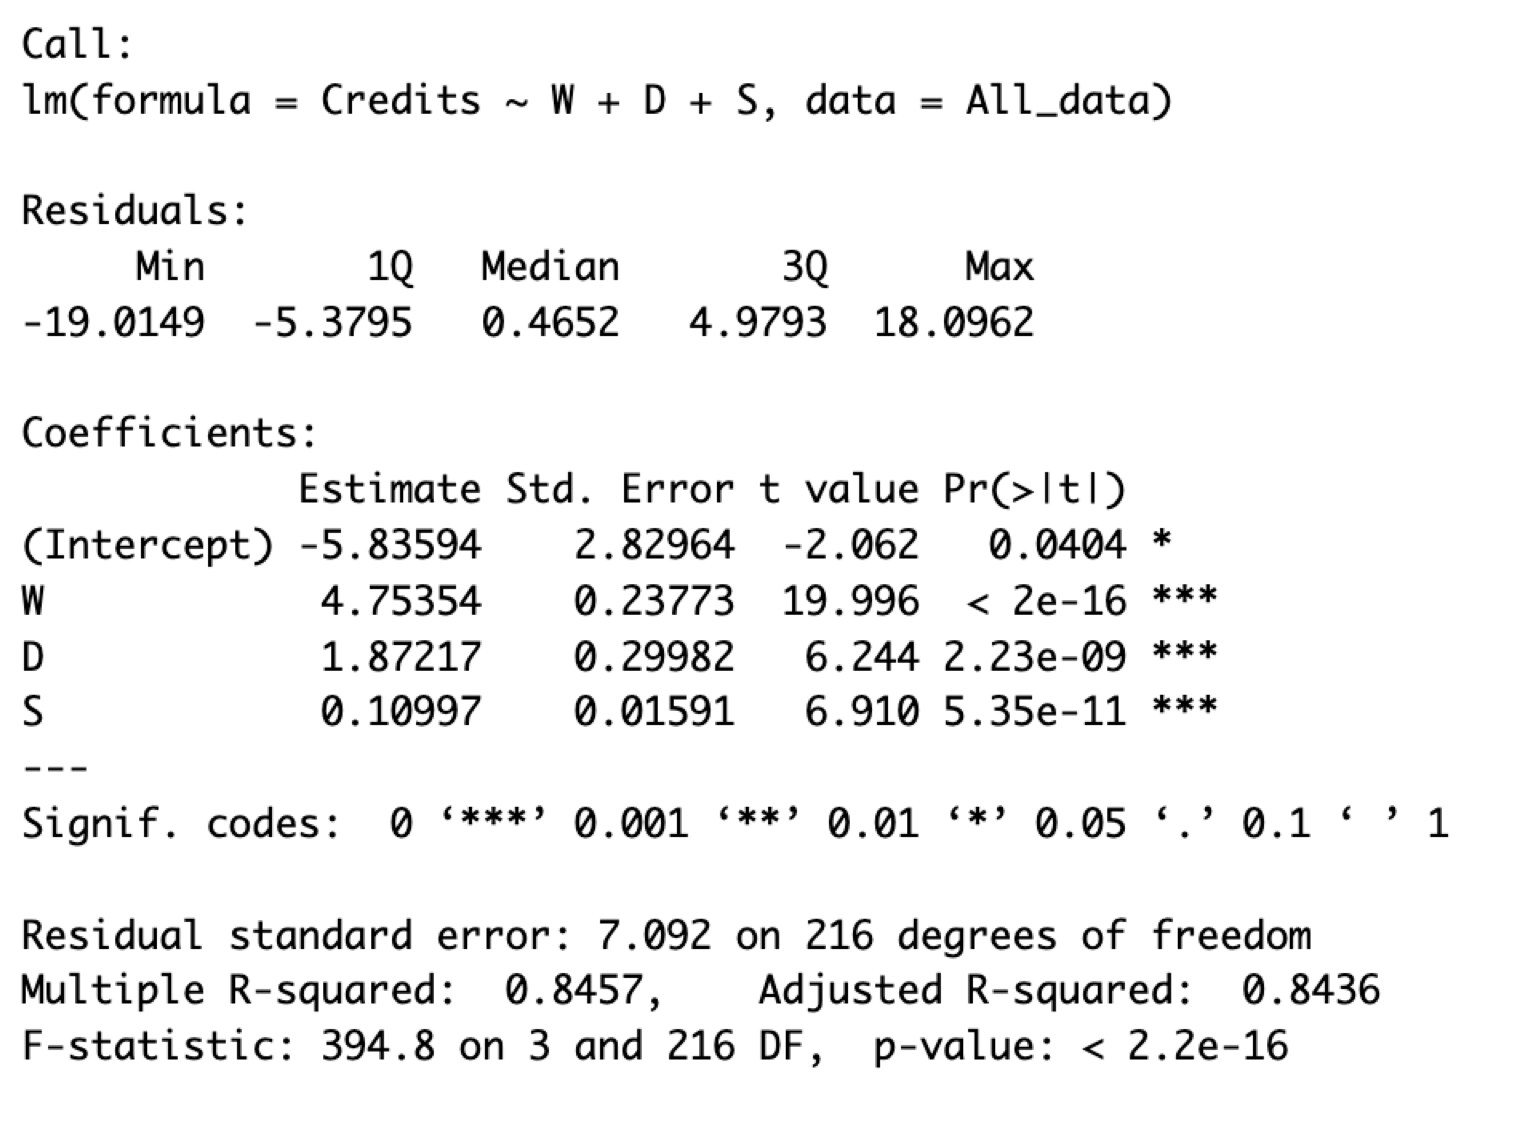
\includegraphics[width=0.32\linewidth]{m2.png}
    \caption{Model 1 \& 2.}
\end{figure}

\begin{figure}[h]
    \centering
    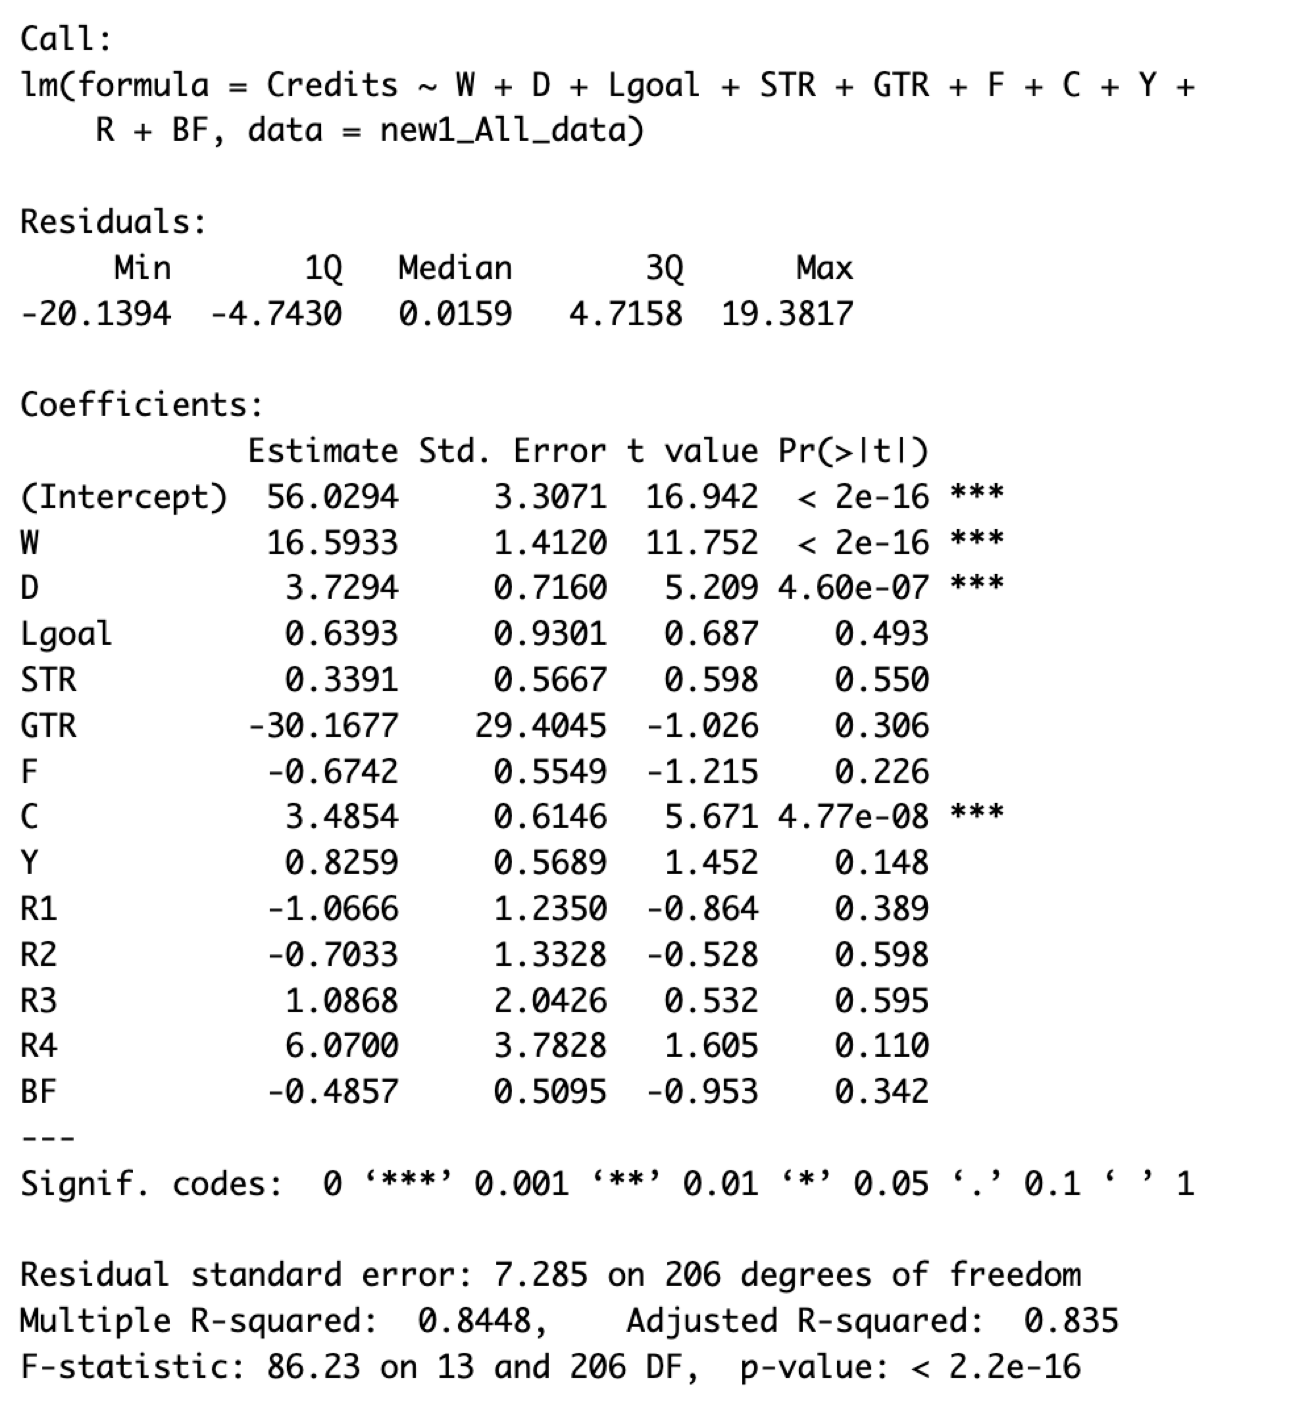
\includegraphics[width=0.32\linewidth]{m3.png}
    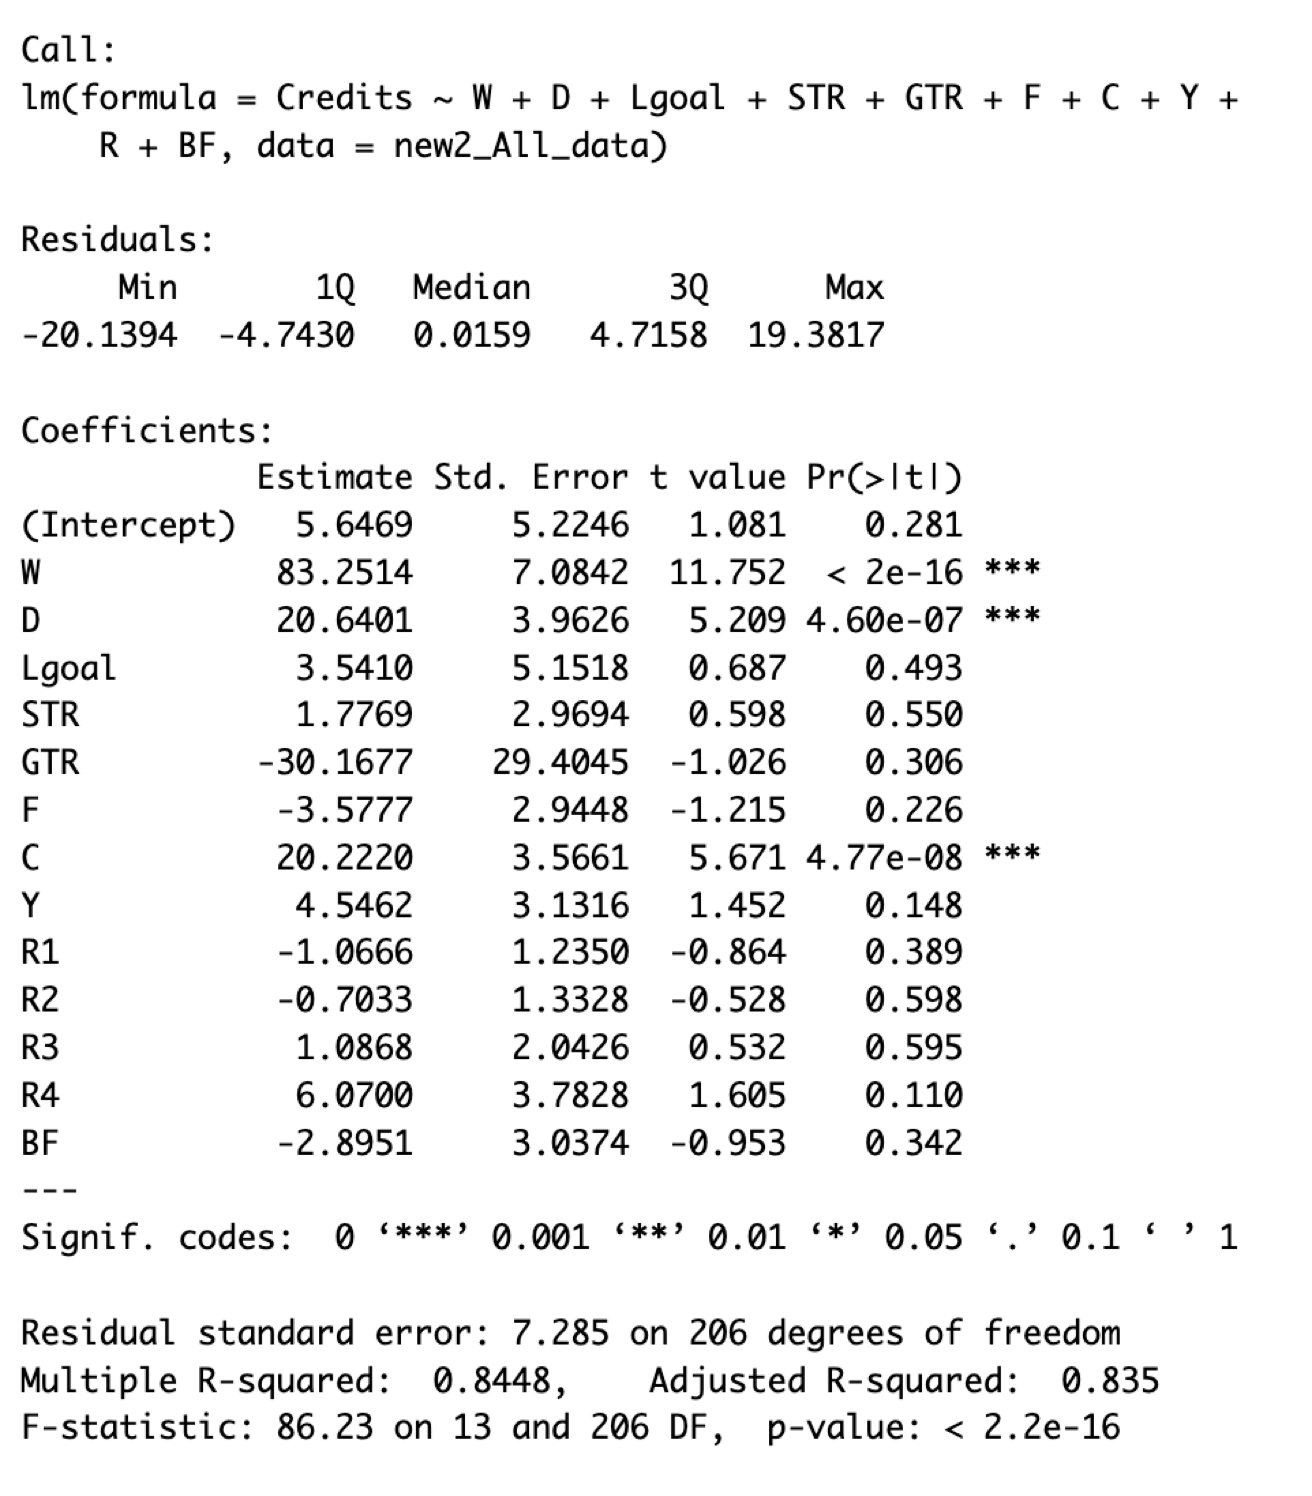
\includegraphics[width=0.32\linewidth]{m4.png}
    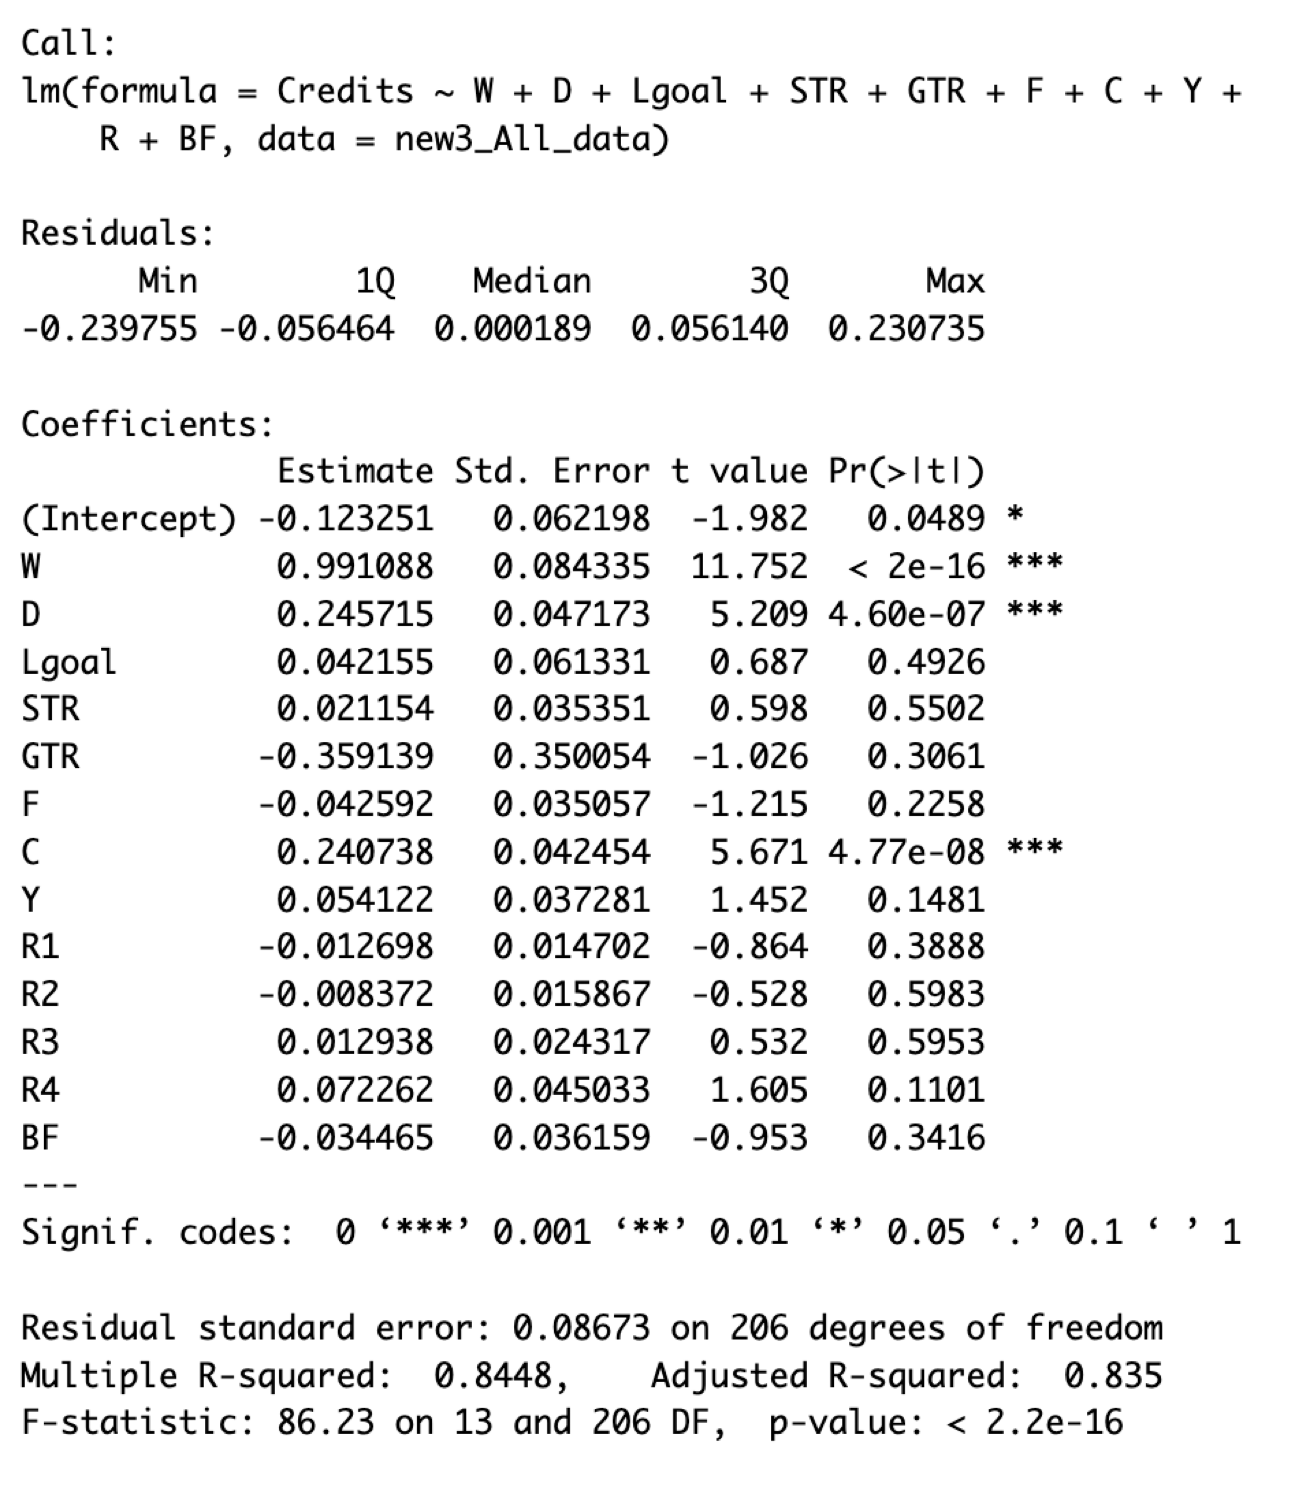
\includegraphics[width=0.32\linewidth]{m5.png}
    \caption{Model 3, 4 \& 5.}
\end{figure}

\newpage
\subsection*{C. MLR Model Prediction}
\label{Prediction}
\begin{figure}[h]
    \centering
    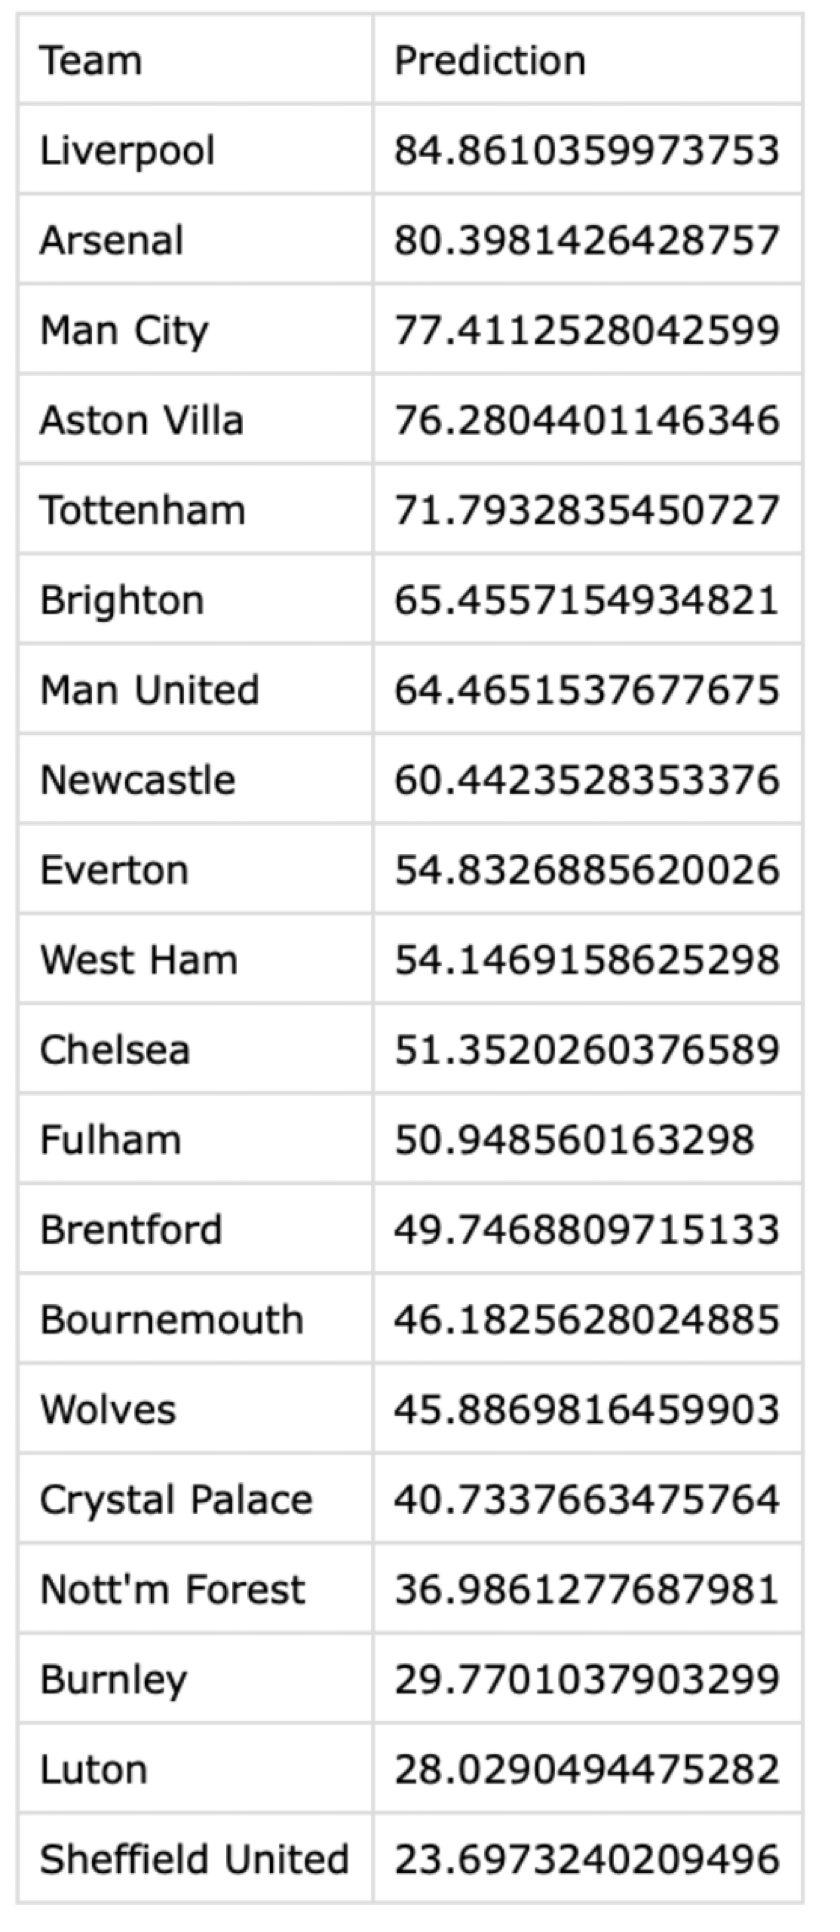
\includegraphics[width=0.32\linewidth]{P1.png}
    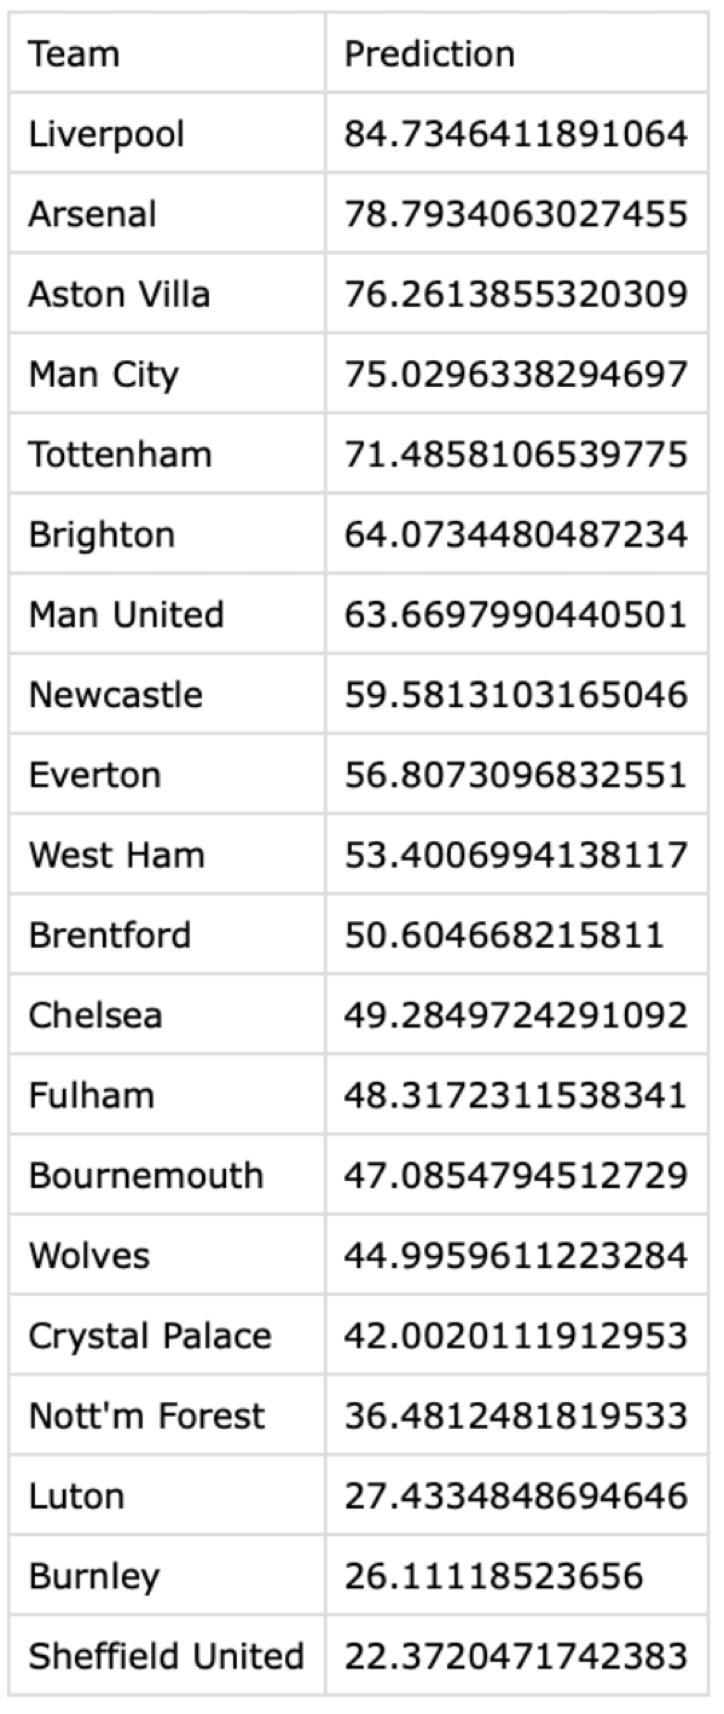
\includegraphics[width=0.32\linewidth]{P2.png}
    \caption{Prediction of Model 1 \& 2.}
\end{figure}
\newpage
\begin{figure}[h]
    \centering
    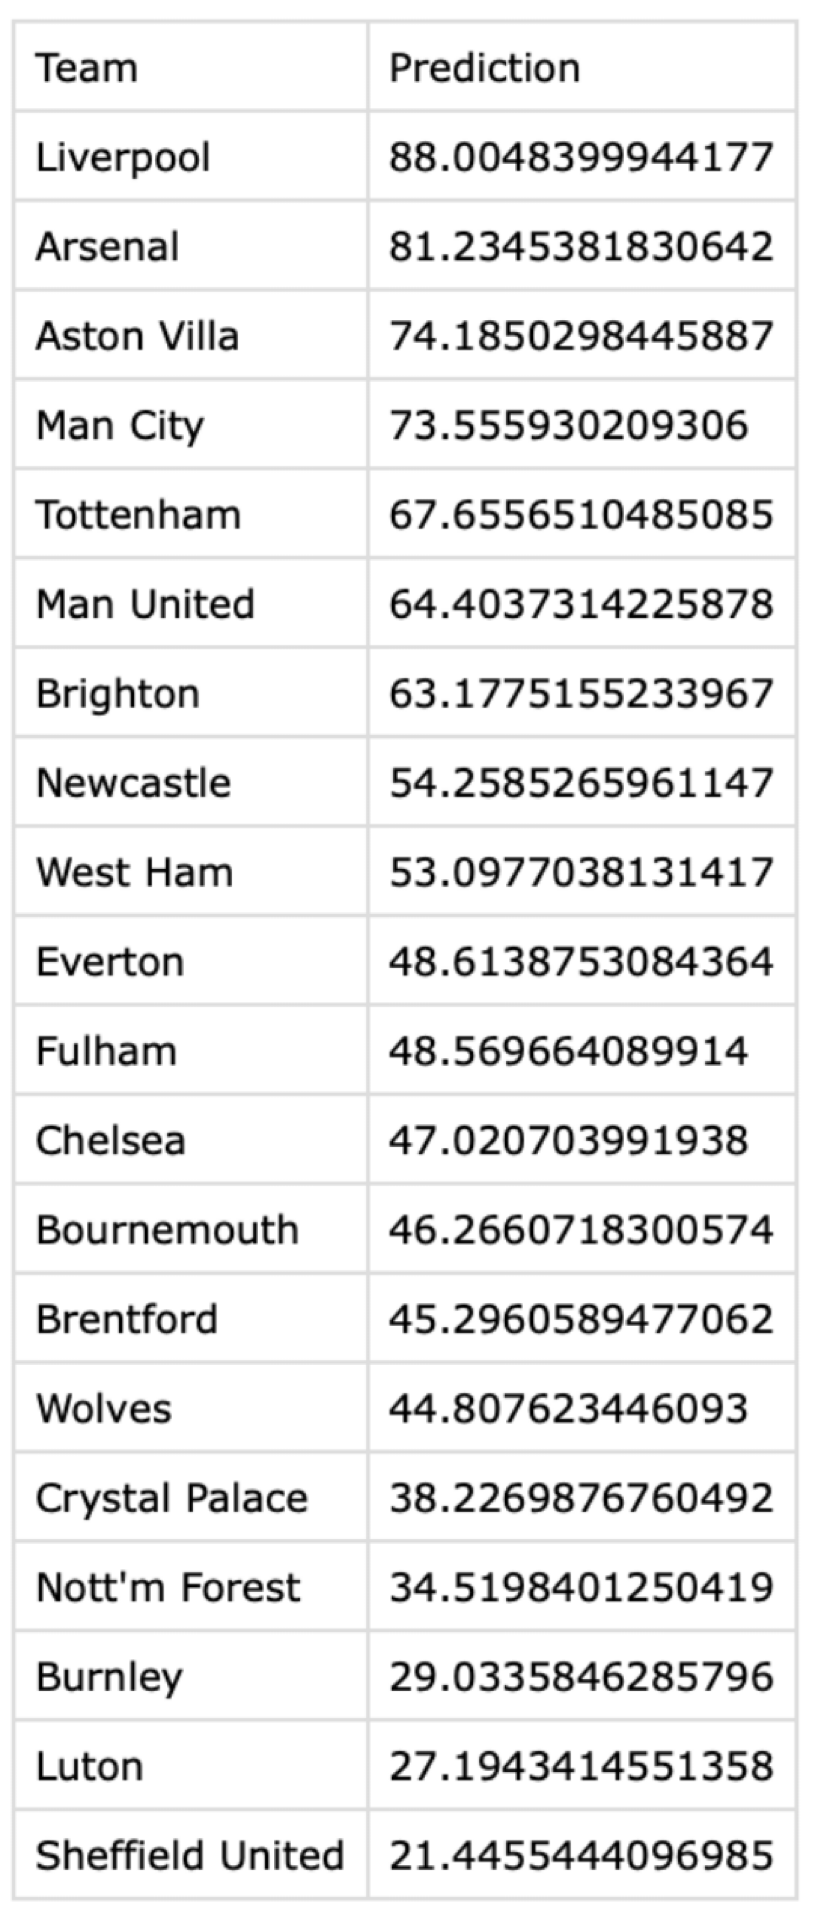
\includegraphics[width=0.32\linewidth]{P3.png}
    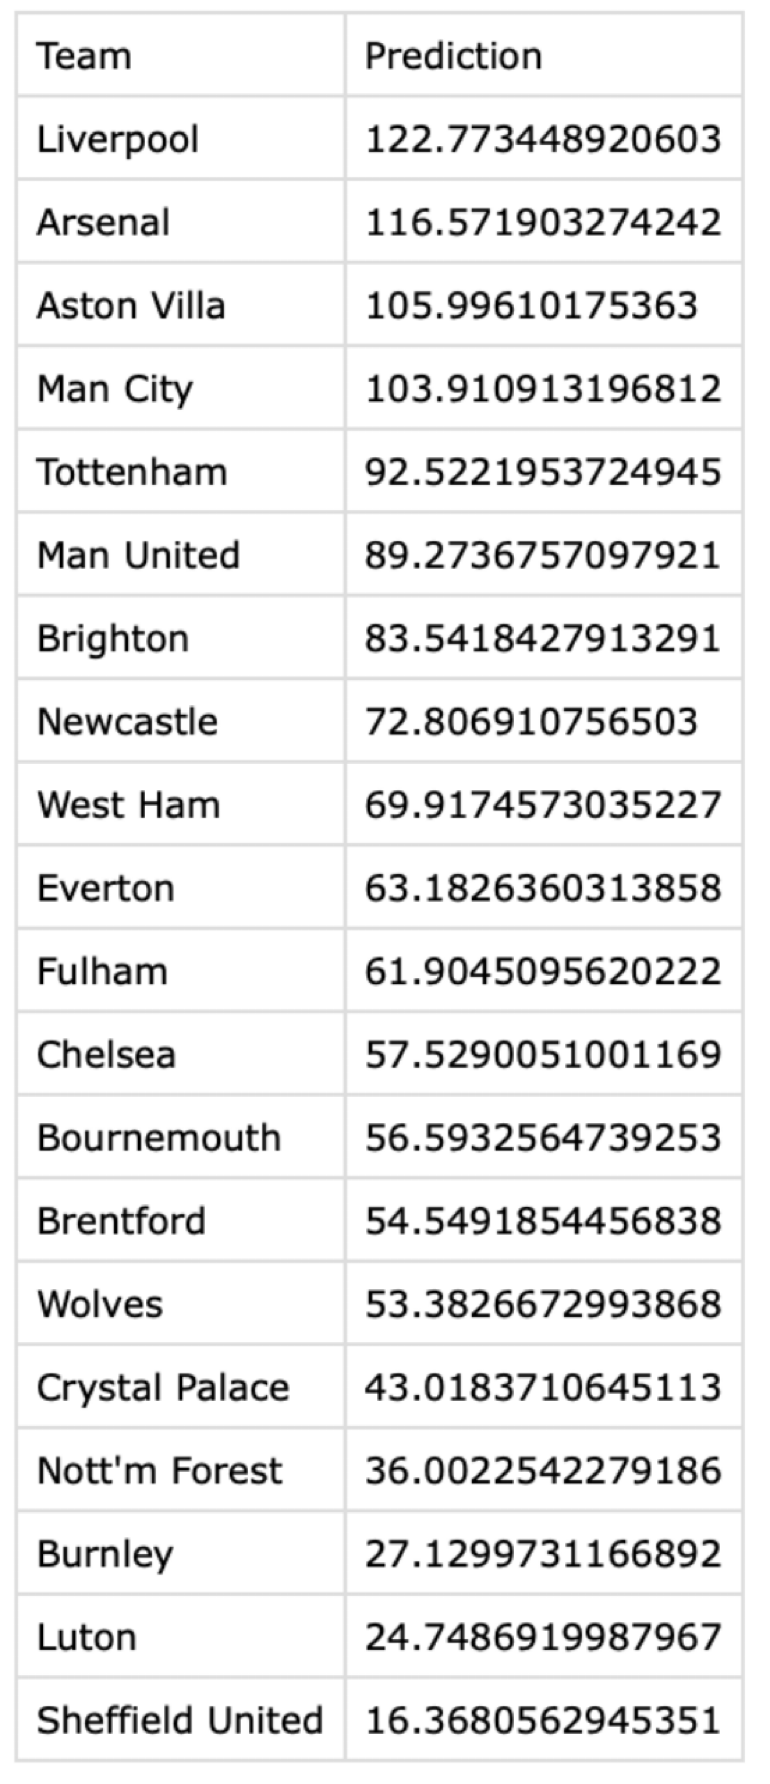
\includegraphics[width=0.32\linewidth]{P4.png}
    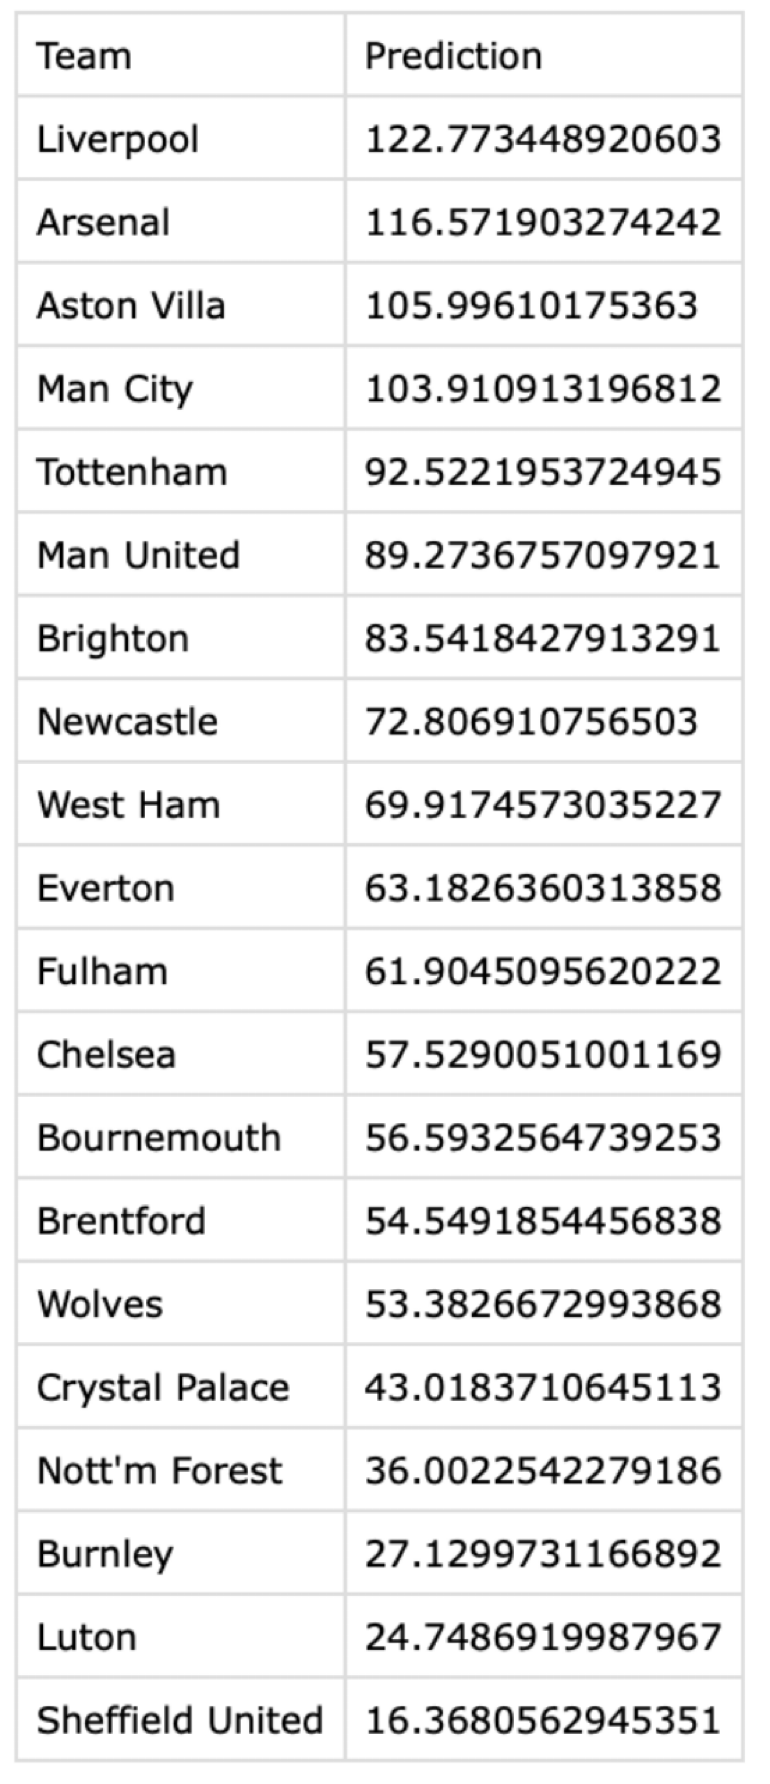
\includegraphics[width=0.32\linewidth]{P5.png}
    \caption{Prediction of Model 3, 4 \& 5.}
\end{figure}


\newpage
\subsection*{D. Prediction of Each Game}
\label{EachGame}
\begin{figure}[h]
    \centering
    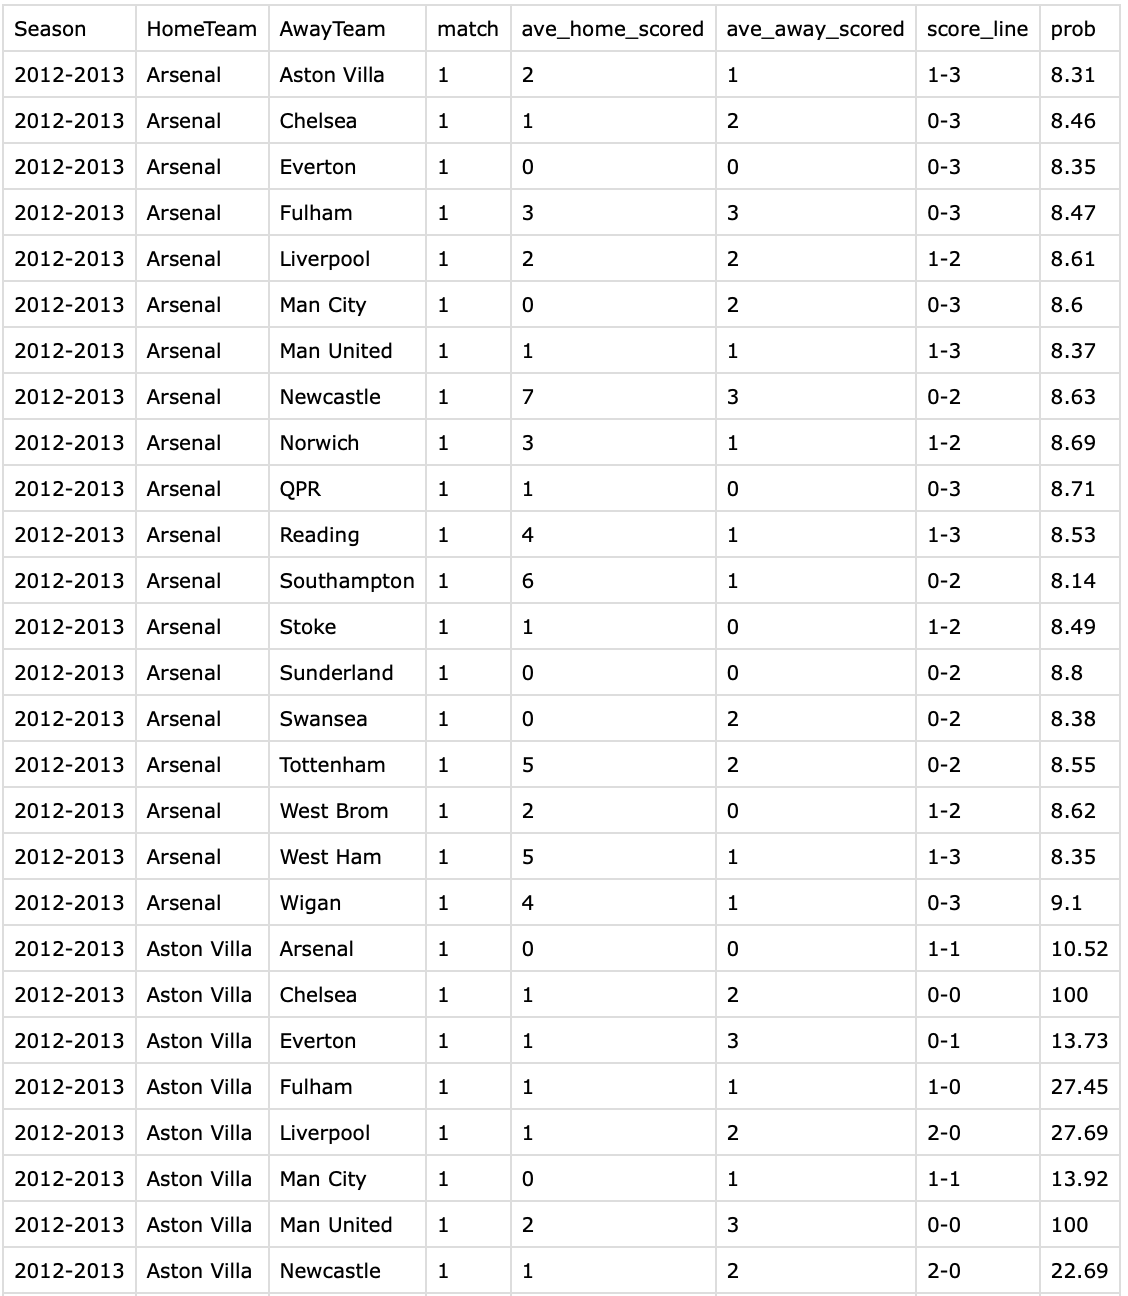
\includegraphics[width=0.8\linewidth]{EG.png}
    \caption{Prediction of Model 3, 4 \& 5.}
\end{figure}
\end{document} 

% \begin{figure}[htb]
% \centering
% \subfloat[Indoor Temperature.]{
% 		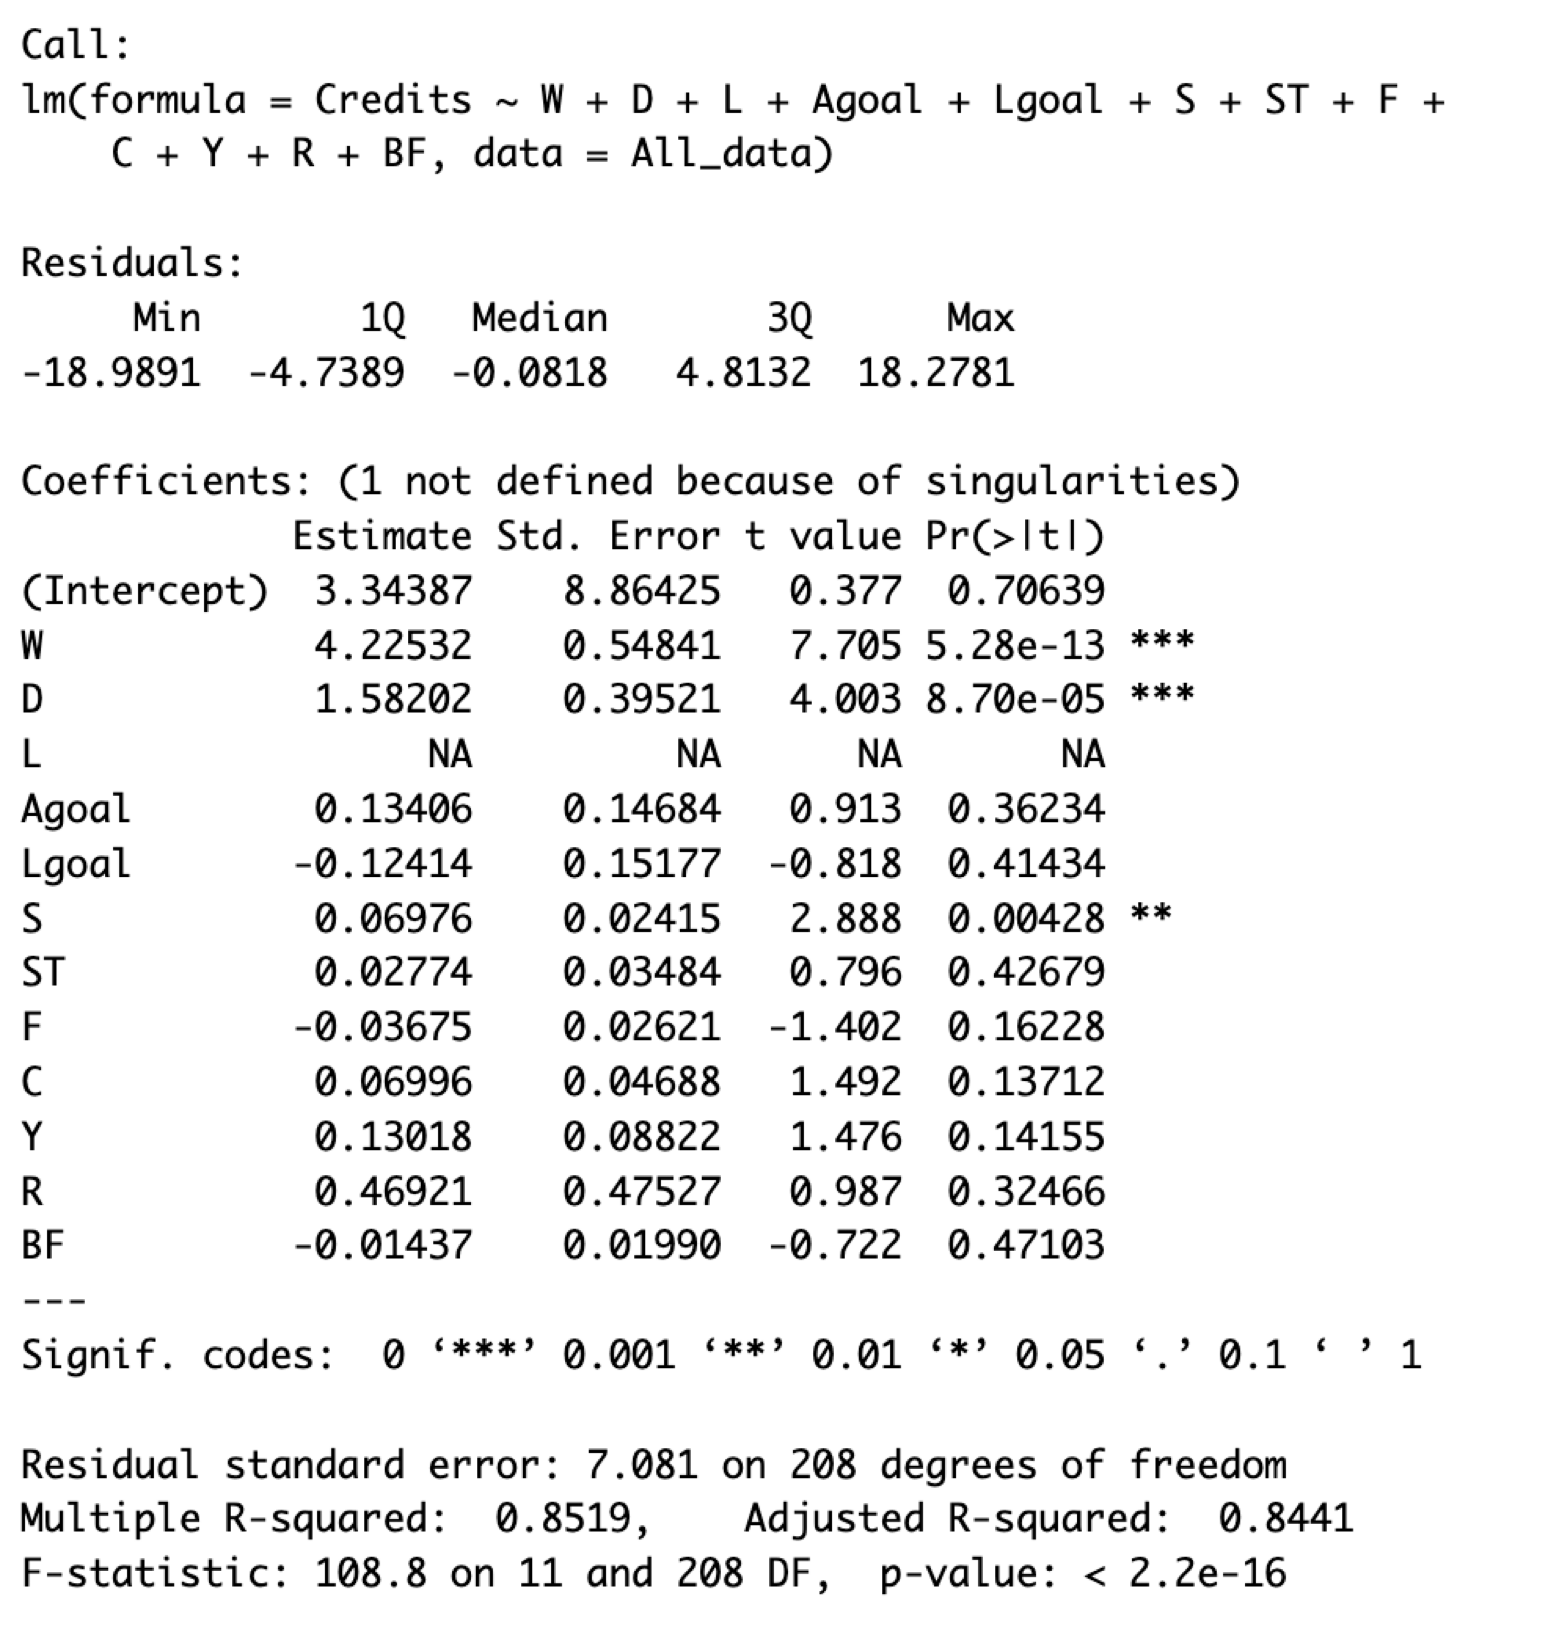
\includegraphics[scale=0.2]{m1.png}}
% \subfloat[Refrigerator Temperature.]{
% 		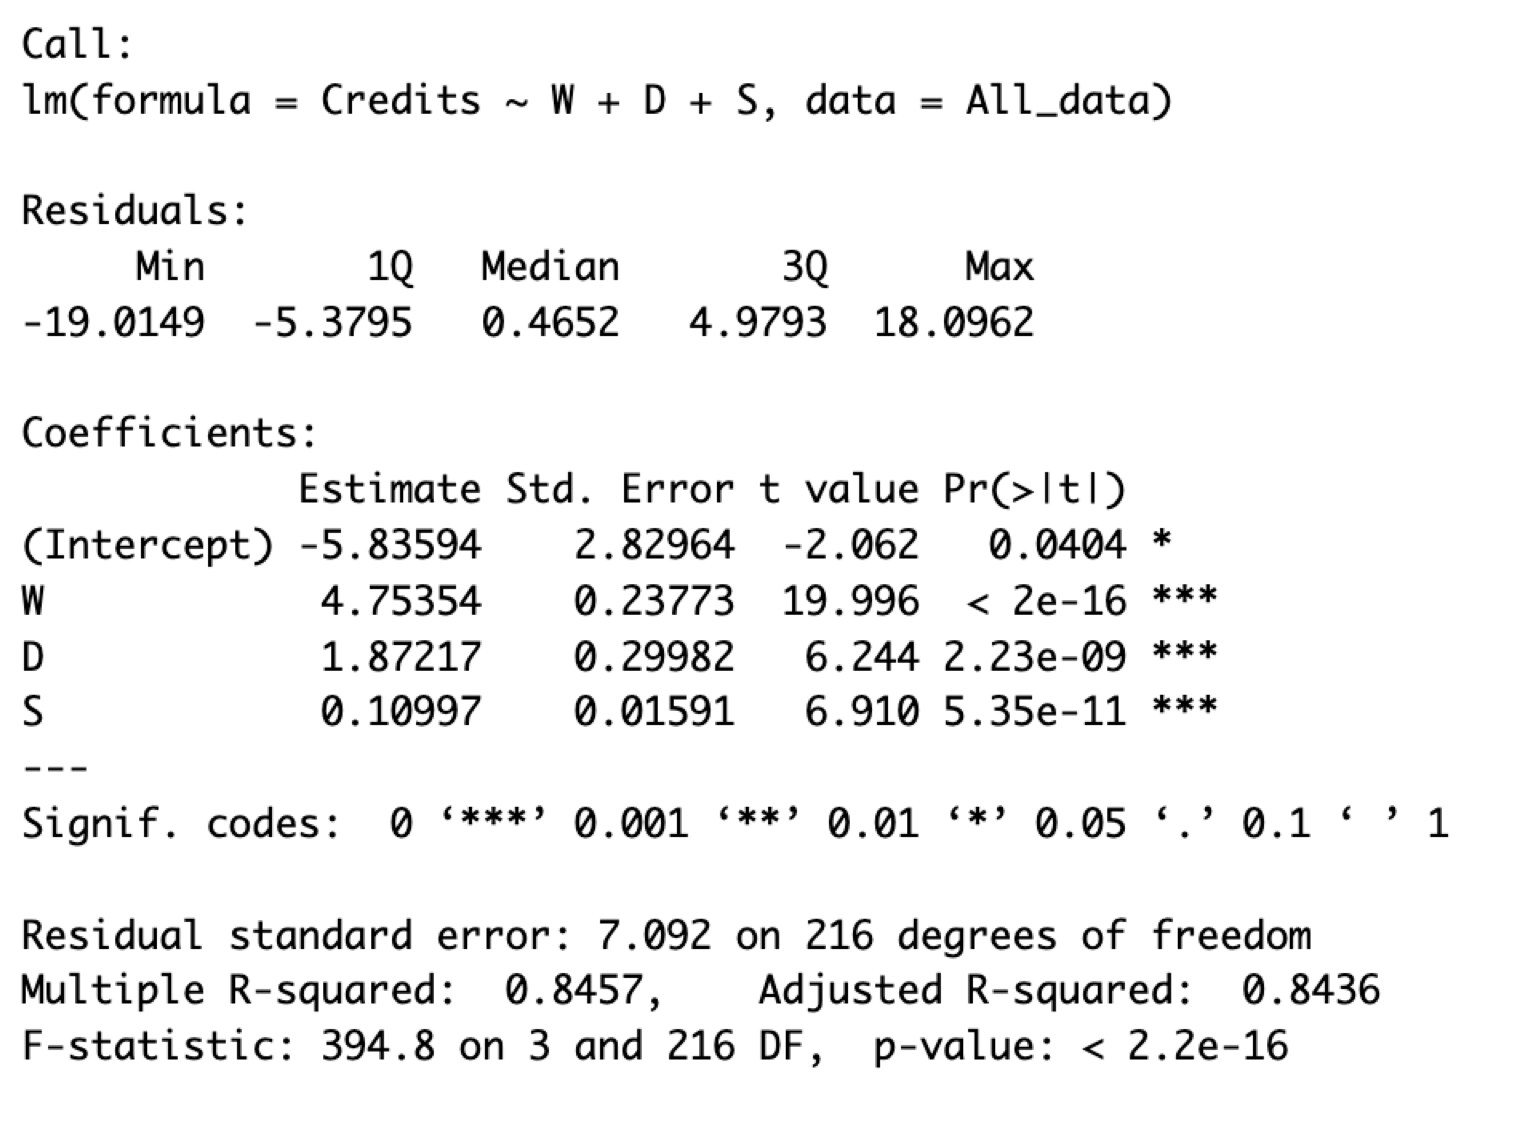
\includegraphics[scale=0.2]{m2.png}}
% \subfloat[Indoor Temperature.]{
% 		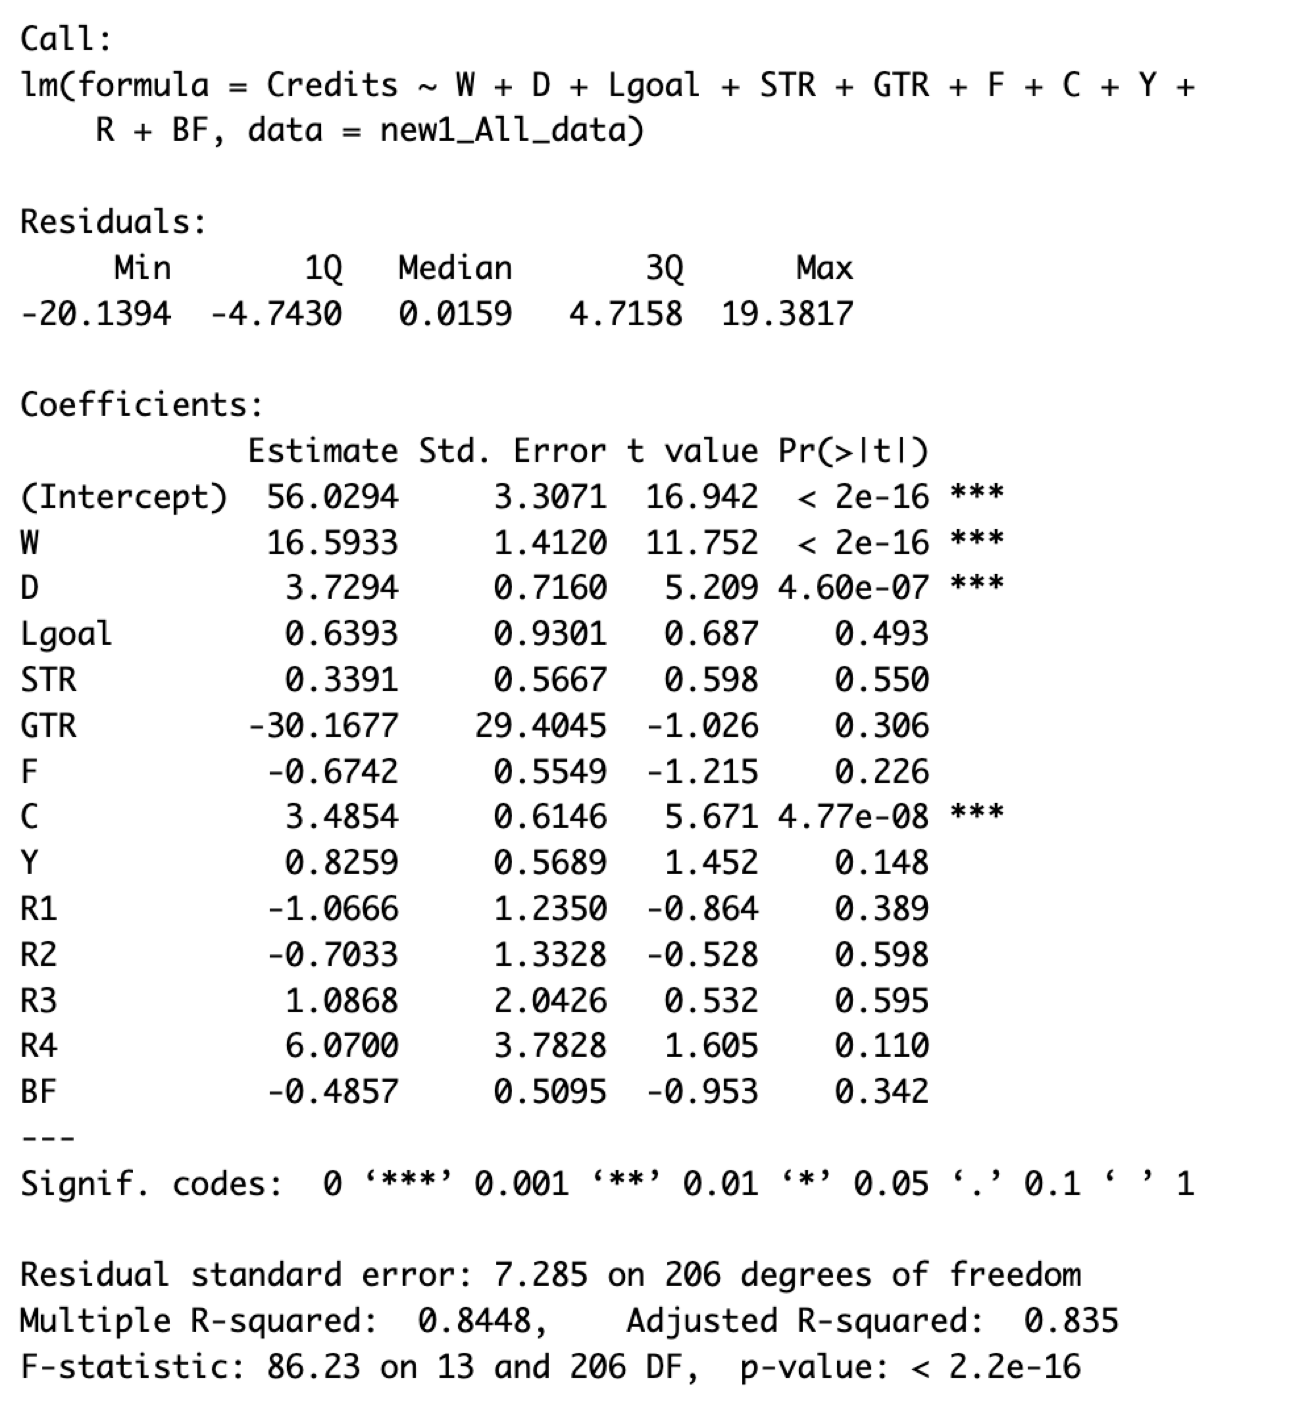
\includegraphics[scale=0.2]{m3.png}}
% \subfloat[Refrigerator Temperature.]{
% 		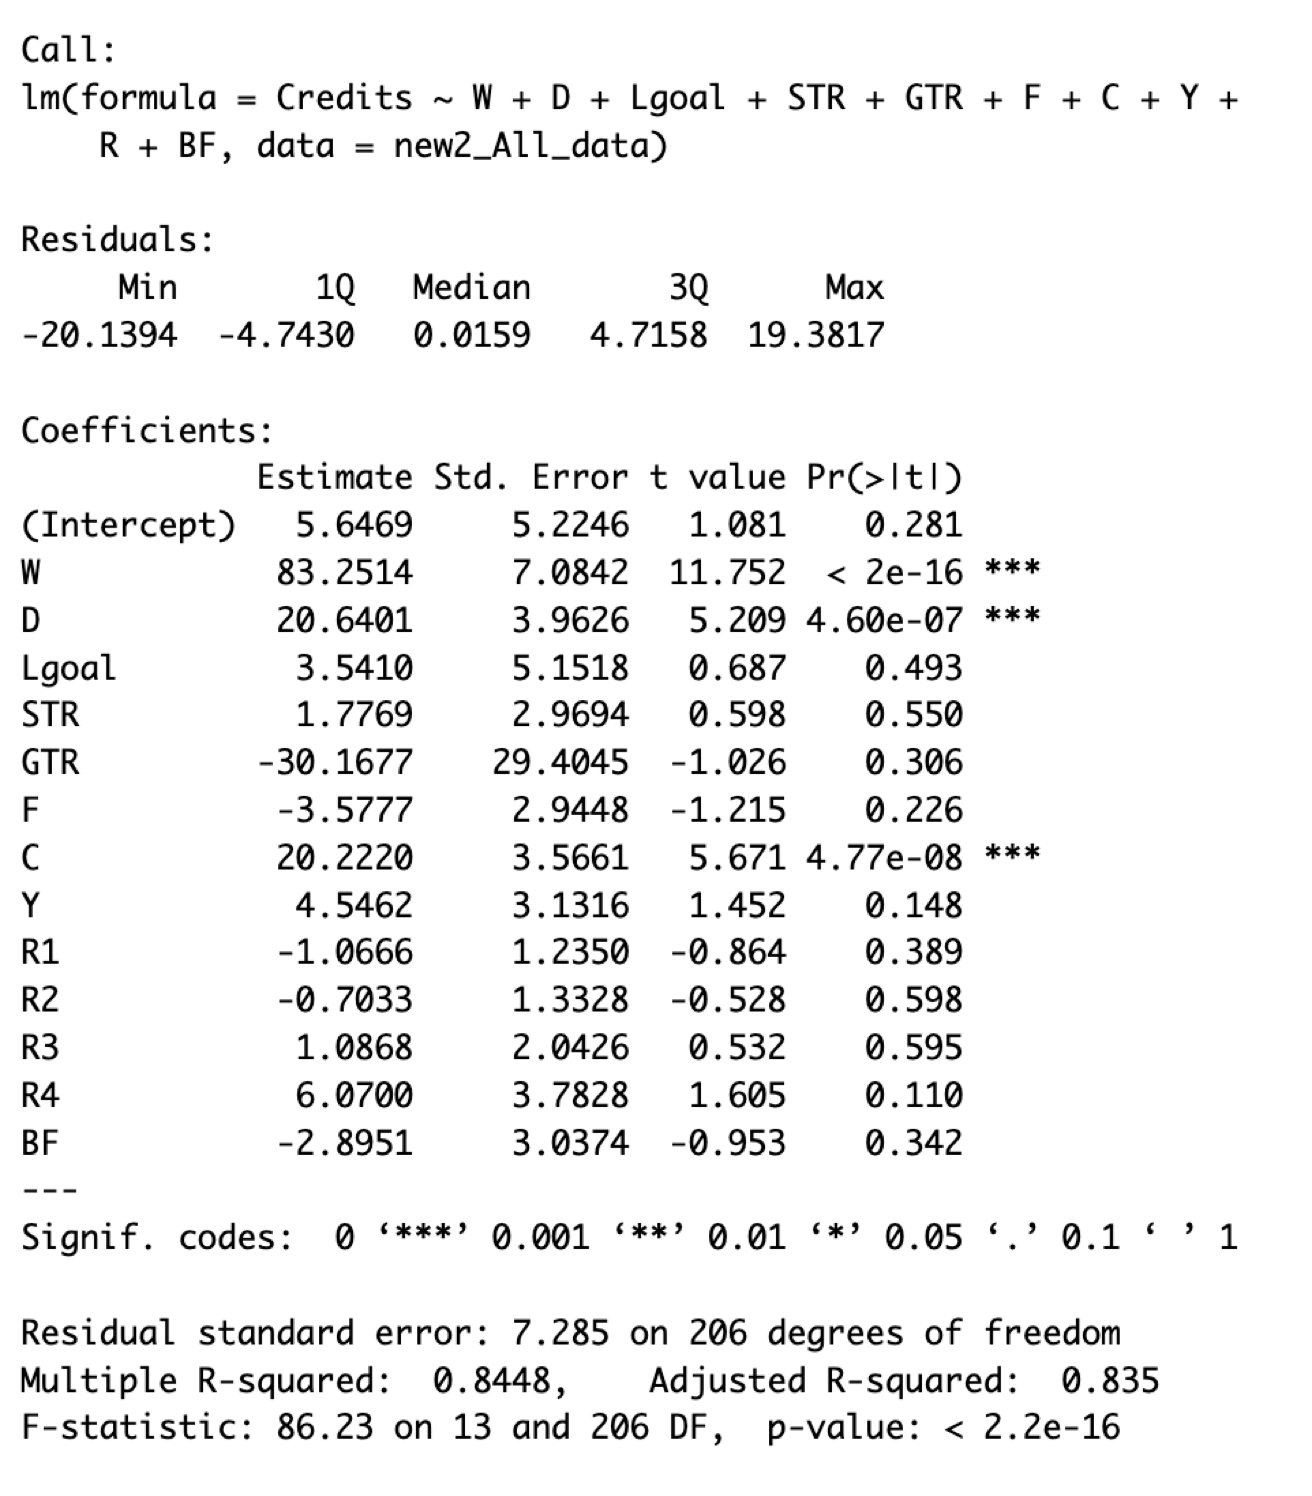
\includegraphics[scale=0.2]{m4.png}}
% \subfloat[Refrigerator Temperature.]{
% 		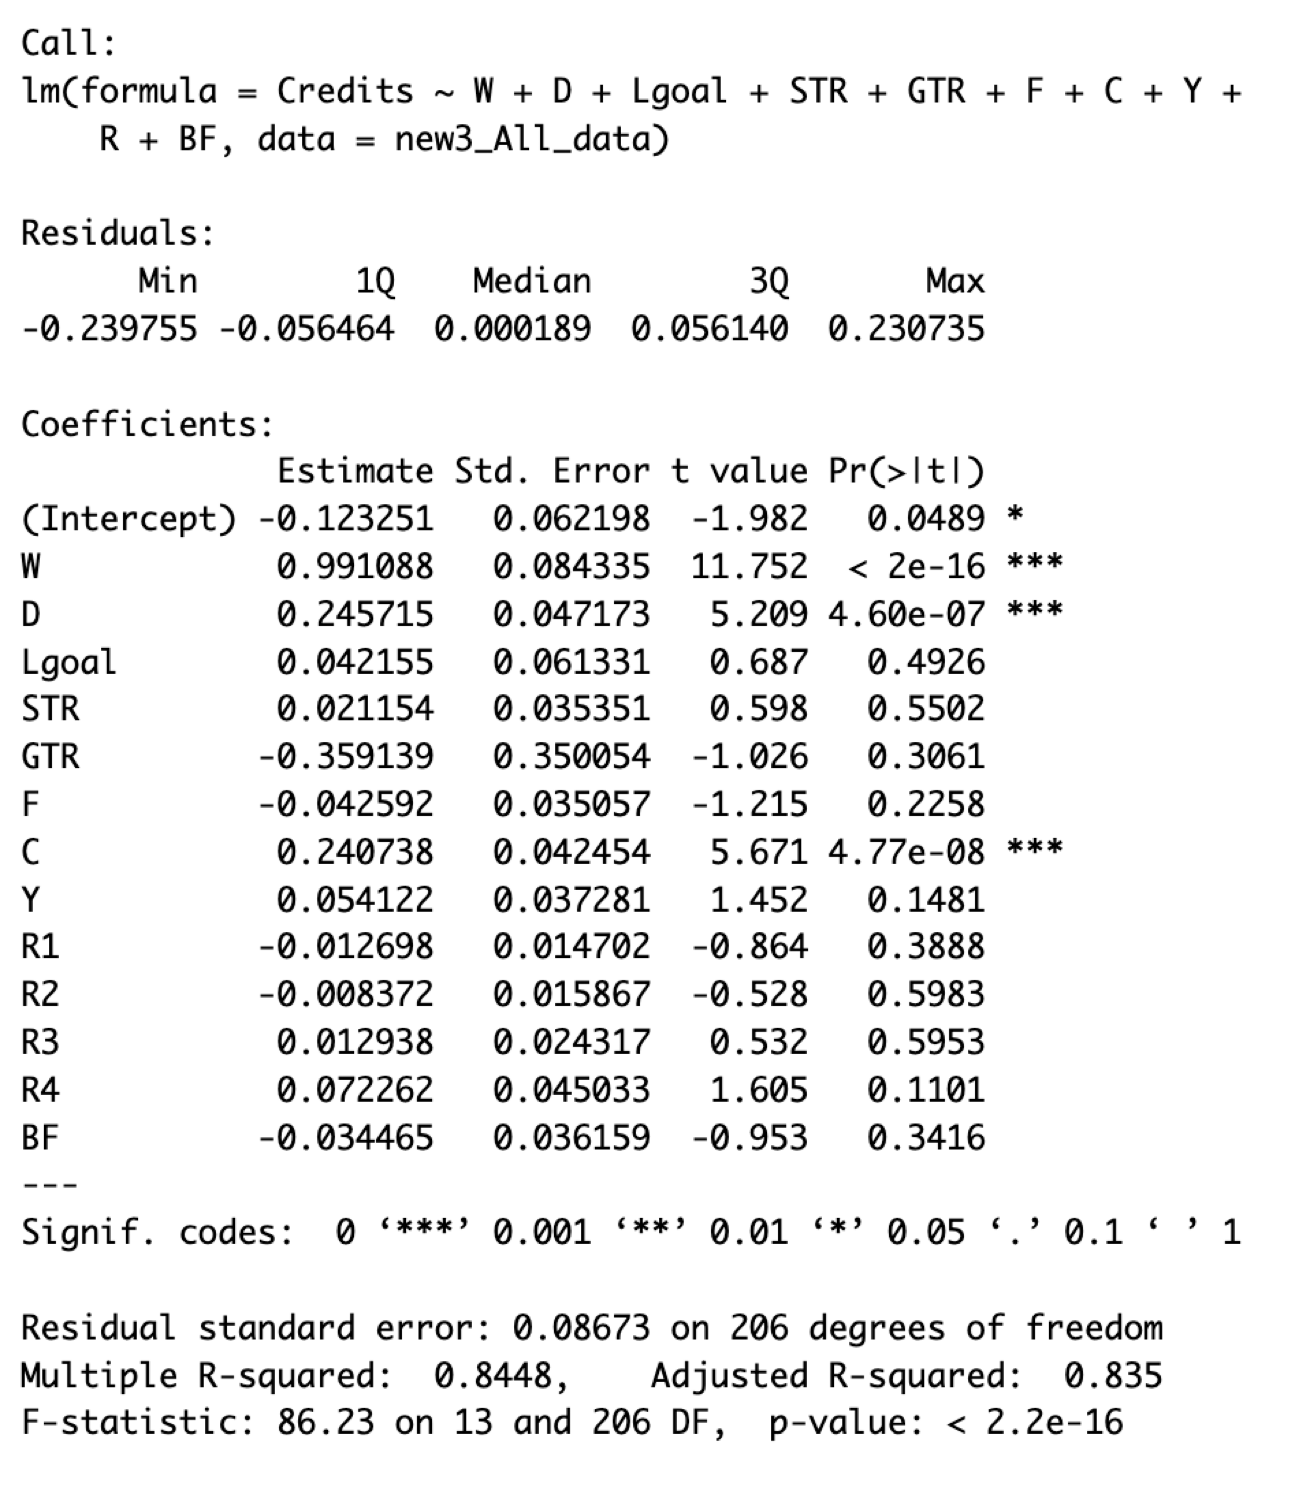
\includegraphics[scale=0.2]{m5.png}}
% \caption{Measured Temperature.}
% \end{figure}